\documentclass[10pt,a4paper]{article}
\usepackage[utf8]{inputenc}
\usepackage[english,russian]{babel}
\usepackage{cmap}
\usepackage[OT1]{fontenc}
\usepackage{amsmath}
\usepackage{amsfonts}
\usepackage{amssymb}
\usepackage{graphicx}
\usepackage{float}
\usepackage{wrapfig}
\usepackage{caption}
\DeclareCaptionLabelSeparator{dot}{. }
\captionsetup{justification=centering,labelsep=dot}
\graphicspath{{pictures/}}
\DeclareGraphicsExtensions{.pdf,.png,.jpg,.eps}
\begin{document}

 

\textbf{11 Алгоритм GraphSLAM}\\

\textbf{11.1	Введение}\\

Алгоритм EKF SLAM, описанный в предыдущих главах, имеет ряд ограничений. Одним из них является квадратичная сложность обновления, а вторым – метод линеаризации в EKF, который выполняется только раз для каждого нелинейного члена. В этой главе будет представлен альтернативный алгоритм SLAM под названием GraphSLAM. В отличие от EKF, GraphSLAM решает полную задачу SLAM и вычисляет оффлайновое решение для  задачи, определённой для всех положений и всех признаков на карте.\\ 
РАЗРЕЖЕНЫЙ ГРАФ\\
Как будет показано в этой главе, апостериорное распределение для \textit{полной задачи SLAM} естественным образом формирует \textit{разреженный граф}. Этот граф сводится к сумме нелинейных квадратичных ограничений, оптимизация которых даст карту максимального правдоподобия и соответствующий набор положений робота. Исторически, эта идея присутствовала в большом числе публикаций по SLAM. Название “GraphSLAM” было отражает основную идею метода.

На Рис. 11.1 показан алгоритм GraphSLAM. Здесь приведён граф, который с помощью GraphSLAM извлекается из пяти положений, отмеченных $x_0,..., x_4$, и двух признаков карты $m_1, m_2$. На графике показаны дуги для движения и измерения. Дуги движения связывают два последующих положения робота, а дуги измерения связывают положения с признаками, наблюдаемыми из данных положений. Каждое ребро графа соответствует нелинейному ограничению. Как будет показано далее, эти ограничения выражают отрицательный логарифм правдоподобия моделей измерения и движения, поэтому лучше всего воспринимать их как информационные ограничения. Добавление такого ограничения к графу в SLAM должно быть тривиально и не требовать существенных вычислений. \\
НАИМЕНЬШИЕ КВАДРАТЫ\\
Сумма всех ограничений даёт нелинейную задачу \textit{наименьших квадратов}, как показано на Рис. 11.1.

Для вычисления апостериорного распределения карты в GraphSLAM выполняется линеаризация набора ограничений. Результатом линеаризации становится информационная матрица и информационный вектор практически того же вида, с которым мы уже сталкивались в Главе 3 при обсуждении информационного фильтра. Однако, информационная матрица наследует свойство разрежённости графа, сконструированного в GraphSLAM. Эта разрежённость позволяет использовать в GraphSLAM алгоритм удаления переменных, и получить граф значительно меньшего размера, определённый только по положению робота. Апостериорная карта пути вычисляется стандартными методами. GraphSLAM также вычисляет карту и определённые маргинальные апостериорные распределения на ней. Полное апостериорное распределение по карте квадратично зависит от размера карты, и восстанавливать его нецелесообразно.

\begin{figure}[H]
	\center{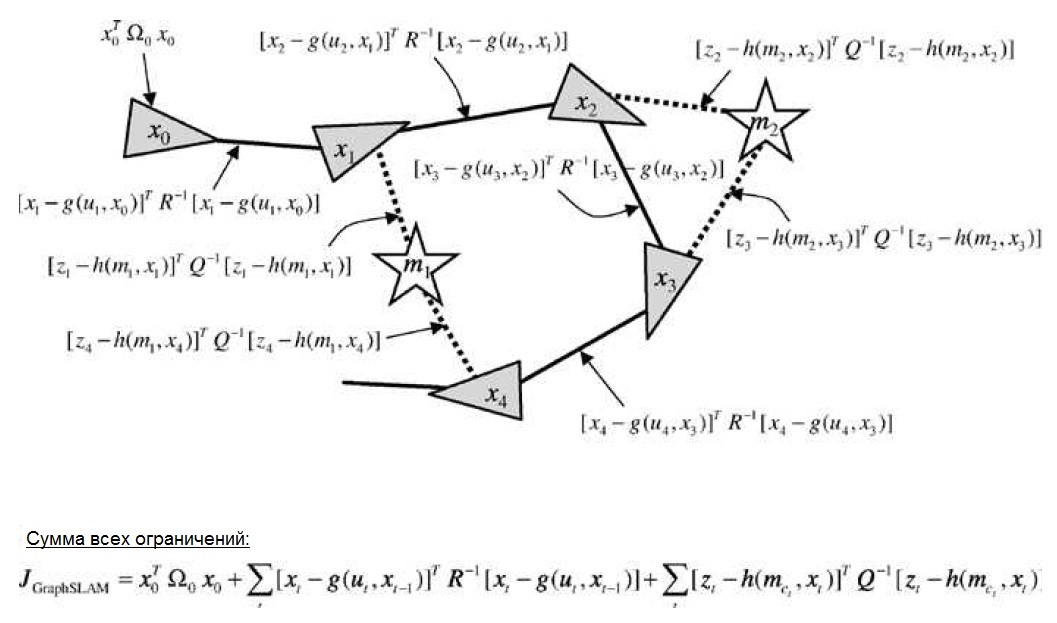
\includegraphics[width=0.9\linewidth]{111orig}}
	\caption{ ( Рис. 11.1  Иллюстрация GraphSLAM для четырёх положений робота и двух признаков карты.  Узлами графа обозначаются положения робота и местоположения признаков. На графе имеется два типа рёбер: сплошными рёбрами обозначены последовательные переходы положений, а пунктирные соединяют положения с признаками, которые робот воспринимает из указанного положения. Каждая связь в GraphSLAM представляет собой нелинейное квадратичное ограничение. Ограничения движения интегрируются в модель движения, а ограничения измерения – в модель измерения, соответственно. Целевой функцией GraphSLAM является сумма этих ограничений, а минимизация этой суммы представляет собой наиболее вероятную карту и самый вероятный путь робота.)}
	\label{fig:111orig}
\end{figure}

Во многих отношениях EKF SLAM и GraphSLAM находятся на противоположных концах семейства алгоритмов SLAM. Основным различием между EKF SLAM и GraphSLAM является способ выражения информации. В  EKF SLAM информация выражается с помощью матрицы ковариации и вектора средних, а в GraphSLAM информация выражается в виде графа мягких ограничений. Обновление ковариации в EKF вычислительно затратно, в то время, как наращивание графа выполняется крайне просто!

Такая экономия тоже имеет свою цену. В GraphSLAM требуются дополнительные преобразования для восстановления карты и пути, а EKF поддерживает наилучшую оценку для карты и положения робота в произвольный момент времени. После построения графа выполняется отдельный такт вычислений, в котором информация преобразуется в оценку состояния.  Для EKF SLAM такой шаг не требуется.\\

ПРОАКТИВНЫЙ SLAM\\

В силу этого можно воспринимать EKF как \textit{проактивный алгоритм SLAM}, поскольку он немедленно разрешает каждую новую порцию информации в улучшенную оценку состояния окружающего мира.\\

ЛЕНИВЫЙ SLAM\\

GraphSLAM, напротив, \textit{ленивый метод SLAM}, который просто аккумулирует информацию в графе, не используя ее. Эта разница существенна, поскольку, в результате, GraphSLAM способен поддерживать карты на много порядков превышающие по размеру те, что способен обработать EKF.

Существуют и другие различия между EKF SLAM и GraphSLAM. Для решения полной задачи SLAM алгоритм GraphSLAM вычисляет апостериорные распределения по траекториям робота, поскольку не является инкрементным алгоритмом. Этот подход отличается от EKF SLAM, который, как и фильтр, сохраняет только апостериорную оценку текущего положения робота. EKF SLAM позволяет роботу произвольно обновлять карту, а GraphSLAM лучше всего подходит для случаев, когда необходимо получить карту из набора данных фиксированного размера. EKF SLAM может сохранять карту в течение всего жизненного цикла робота, без необходимости учитывать общее число тактов времени, прошедших с момента начала получения данных.

Поскольку GraphSLAM при построении карты имеет доступ ко всем данным, в нем можно использовать улучшенные методы ассоциации данных и линеаризации. В EKF SLAM, линеаризация и соответствие в момент времени $t$ вычисляются на основе карты, полученной вплоть до предыдущего момента. В GraphSLAM для линеаризации и вычисления соответствия используются все имеющиеся данные. Другими словами, GraphSLAM способен пересмотреть уже выполненную в прошлом ассоциацию данных и выполнить линеаризацию несколько раз. Фактически, в GraphSLAM последовательно выполняется три критических шага картографирования: создание карты, вычисление переменных соответствия и линеаризацию моделей измерения и движения, что позволяет получить наиболее точные оценки их значений. В результате этого GraphSLAM часто создаёт карты, превосходящие по точности EKF.

Однако, GraphSLAM имеет ряд ограничений по сравнению с EKF. Одно из них уже обсуждалось: размер графа линейно растёт со временем, а в EKF нет такой зависимости количества занимаемой оценками памяти от времени. Другой случай относится к ассоциации данных. Если в EKF SLAM вероятности ассоциации данных легко получить из матрицы ковариации апостериорного распределения, вычисление тех же вероятностей в GraphSLAM требует дополнительных выводов. Эта разница будет описана ниже, в разделе определении алгоритма вычисления соответствия в GraphSLAM. Поэтому, вопрос наилучшей применимости метода не имеет чёткого ответа и зависит от области применения, поскольку ни один метод не будет превосходить остальные по всем критическим показателям. 

В этой главе сначала описывается основная идея GraphSLAM и основные такты обновления. Затем будет представлен математический вывод различных тактов обновления и доказана их правильность относительно конкретных линейных аппроксимаций. Также будет выведен метод ассоциации данных, а затем – приведено обсуждение конкретных реализаций алгоритма GraphSLAM.\\

\textbf{11.2	Общее описание}\\

Основная идея, лежащая в основе GraphSLAM, достаточно проста: из данных извлекается  набор мягких ограничений, который отображается в виде разреженного графа. Карта и траектория робота получаются в результате разрешения этих ограничений в виде глобально непротиворечивой оценки. Ограничения, в общем случае, имеют нелинейный вид, но в процессе разрешения линеаризуются и преобразуются в информационную матрицу. В силу этого, GraphSLAM представляет собой, в основном, информационно-теоретический метод. Мы опишем GraphSLAM как в виде метода построения разреженного графа нелинейных ограничений, так и в виде метода распространения разреженной информационной матрицы линеаризованных ограничений.\\

\textbf{11.2.1	Построение графа}\\

Допустим, дан набор измерений $z_{1:t}$ со связанными переменными соответствия $c_{1:t}$ и набором управляющих воздействий $u_{1:t}$. GraphSLAM превращает эти данные в граф, узлы которого представляют положения робота $x_{1:t}$ и признаки карты $m = \{m_j\}$. Каждое ребро графа соответствует некоторому событию: событие движения создаёт ребро между двумя положениями робота, а событие измерения связывает положение робота и признак на карте. Ребра выражают мягкие ограничения между положениями робота и признаками в GraphSLAM.

Для линейной системы эти ограничения эквивалентны элементам информационной матрицы и информационного вектора большой системы уравнений. Как обычно, обозначим информационную матрицу через $\varOmega$, а информационный вектор -через $\xi$. Как будет показано ниже, каждое измерение и каждое управляющее воздействие приводят к локальному обновлению $\varOmega$ и $\xi$, что соответствует локальному добавлению ребра графа в GraphSLAM. Фактически, правило учёта управляющего воздействия или измерения в $\varOmega$ и $\xi$ – это локальное добавление, в силу важного факта аддитивности информации. 

На. Рис. 11.2 показан процесс создания графа, а также соответствующая информационная матрица. Сначала учитывается измерение $z_t^i$. Это измерение предоставляет информацию о связи между местоположением признака $j = c_t^i$ и положением робота $x_t$ в момент времени $t$. В GraphSLAM эта информация проектируется в виде ограничения между $x_t$ и $m_j$. Можно описать ребро в виде некой «пружины» по аналогии с кинематической моделью масс, соединённых пружинами. Как будет показано ниже, ограничение имеет вид:\\

(11.1)
$$(z_t^i-h(x_t,m_j))^T\,Q_t^{-1}\,(z_t^i-h(x_t,m_j))$$

Здесь $h$ - уже знакомая функция измерения, а $Q_t$ - ковариация шумов измерения. На Рис. 11.2a показано добавление такой связи в граф, сохраняемый в GraphSLAM.

Теперь необходимо учесть движение робота. Управляющее воздействие $u_t$ даёт информацию об относительном значении положения робота в момент времени $t-1$ и положении в момент времени $t$. И снова, интегрирование этой информации приводит к появлению нового ребра в графе вида\\

(11.2)
$$(x_t-g(u_t,x_{t-1}))^T\,R_t^{-1}\,(x_t-g(u_t,x_{t-1}))$$

Здесь $g$ – уже знакомая кинематическая модель движения робота, а $R_t$ - ковариация шумов движения.

\begin{figure}[H]
	\center{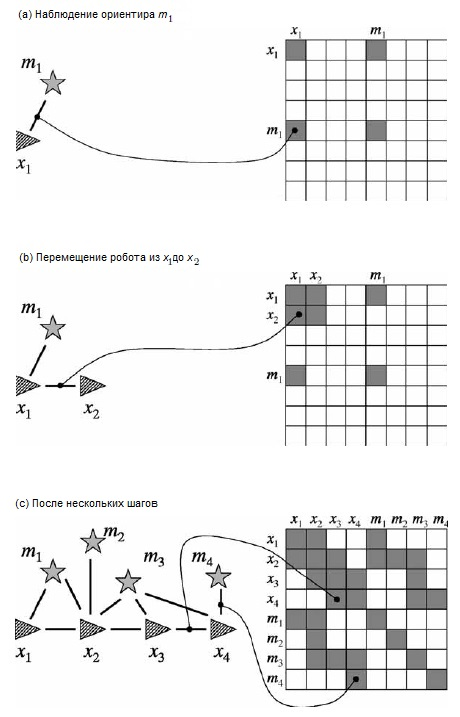
\includegraphics[width=0.9\linewidth]{112orig}}
	\caption{ ( Рис. 11.2 Получение информационной матрицы в GraphSLAM. На левой схеме показан граф зависимостей, на правой – информационная матрица.)}
	\label{fig:112orig}
\end{figure}

На Рис. 11.2b показано добавление такой связи к графу. Также изображено добавление нового элемента связи между положением $x_t$ и измерением $z_t^i$ в информационную матрицу. Эта процедура тоже аддитивна. Как и раньше, величина этих значений отражает остаточную неопределённость $R_t$, вызванную шумами измерений.  Чем точнее датчик, тем большее значение будет добавлено к $\varOmega$ и $\xi$.

После учёта всех измерений $z_{1:t}$ и управляющих воздействий $u_{1:t}$ получим разреженный граф мягких ограничений. Число ограничений в графе линейно зависит от времени, следовательно, граф разрежен. Сумма всех ограничений графа должна иметь вид\\

(11.3)
\begin{equation*}
\begin{split}
J_{\text{GraphSLAM}}=\,&x_0^T\varOmega_0x_0+\sum_t(x_t-g(u_t,x_{t-1}))^T\,R_t^{-1}\,(x_t-g(u_t,x_{t-1}))\\
&+\sum_t\sum_i(z_t^i-h(y_t,c_t^i))^T\,Q_t^{-1}\,(z_t^i-h(y_t,c_t^i))
\end{split}
\end{equation*}

и представляет собой функцию, определённую по переменным положения $x_{1:t}$ и всем расположениям признаков на карте $m$.\\

ФИКСИРУЮЩЕЕ ОГРАНИЧЕНИЕ\\

Заметим, что это выражение также характеризует фиксирующее ограничение вида $x^T_0\,\,\varOmega_0\,\,x_0$. (anchoring  constraint) Это ограничение выполняет привязку абсолютных координат карты путём инициализации первого положения робота в точке $(0\,\,0\,\,0)^T$ .

В связанной информационной матрице $\varOmega$ все элементы вне главной диагонали равны нулю, за исключением двух. Между двумя последовательными положениями $x_{t-1}$ и $x_t$ будет находиться ненулевое значение, выражающее информационную связь, внесённую управляющим воздействием $u_t$. Также ненулевым будет любой элемент между признаком карты $m_j$ и положением $x_t$, для которого $m_j$ можно наблюдать из положения робота $x_t$. Все элементы между прочими парами признаков остаются нулевыми. Это отражает факт отсутствия информации об относительном местоположении, поскольку всё, что поступает на вход SLAM, это измерения, ограничивающие расположение признака относительно положения робота. Поэтому информационная матрица также разрежена, а все элементы, за исключением некоторого линейного количества, равны нулю.\\

\textbf{11.2.2	Соображения}\\

Конечно, ни отображение в виде графа, ни информационная матрица не дают желаемого результата, то есть карты и траектории движения. В GraphSLAM карта и траектория получаются из линеаризованной информационной матрицы с помощью $\mu=\varOmega^{-1}\xi$ (см. Равенство (3.73) на странице 72 ???). Для этой операции требуется решить систему линейных уравнений и возникает вопрос о том, насколько эффективно возможно восстановить оценку карты $\mu$ и ковариацию $\varSigma$.

Ответ на вопрос о сложности зависит от топологии среды. Если каждый признак наблюдается только локально по времени, то и граф, выраженный в виде ограничений, будет линеен. Поэтому $\varOmega$ можно переопределить в виде ленточной матрицы, где все ненулевые элементы расположены вдоль главной диагонали, а уравнение $\mu=\varOmega^{-1}\xi$ можно вычислить за линейное время. Это соображение соответствует неповторяющейся окружающей среде, через которую проходит робот, так что все признаки различимы лишь в течение короткого периода времени, последовательно, один за другим.

Более общий случай, однако, включает признаки, наблюдаемые несколько раз с большими промежутками времени между наблюдениями.\\
ЦИКЛЫ\\
Это может произойти, например, если робот перемещается вперёд и назад по коридору, или в силу наличия в окружающей среде \textit{циклов}. В любом случае, будут существовать признаки $m_j$ наблюдаемые в сильно отличающиеся моменты времени $x_{t_1}$ и $x_{t_2}$, с $t_2\gg t_1$. На графе ограничений это вызывает циклическую зависимость: $x_{t_1}$ и $x_{t_2}$ соединены через последовательность управляющих действий $u_{t_1+1}, u_{t_1+2},..., u_{t_2}$ и через последовательность наблюдений между $x_{t_1}$ и $m_j$, в промежутке  между $x_{t_2}$ и $m_j$, соответственно. Такие связи не позволяют выполнить переопределение переменных, что усложняем восстановление карты. Фактически, поскольку инвертированная $\varOmega$ перемножается с вектором, результат возможно вычислить, используя методы оптимизации, например, сопряжённых градиентов, без необходимости явно вычислять полную обратную матрицу. Поскольку большая часть сред имеет циклы, этот случай представляет интерес.\\

ФАКТОРИЗАЦИЯ\\

В алгоритме GraphSLAM теперь можно выполнить \textit{факторизацию}, который можно считать распространением информации через информационную матрицу (это обобщение известного алгоритма \textit{удаления переменных} для инверсии матрицы). Допустим, хотелось бы удалить признак $m_j$ из информационной матрицы $\varOmega$ и информационного состояния $\xi$. В кинематической модели масс на пружинах это эквивалентно удалению узла массы и всех соединённых с ним пружин. Как мы увидим ниже, это возможно с помощью довольно простой операции: можно «удалить пружины» между $m_j$ и положениями, из которых наблюдался $m_j$, поставив «новые пружины» для каждой пары таких положений.

Этот процесс показан на Рис. 11.3, где показано удаление двух признаков карты, $m_1$ и $m_3$ (удаление $m_2$ и $m_4$ в этом примере тривиально). В обоих случаях, удаление признаков изменяет связь в каждой паре положений, из которых наблюдался признак. Как показано на Рис. 11.3b, эта операция может привести к возникновению новых связей в графе. В показанном примере удаление $m_3$ приводит к появлению новой связи между $x_2$ и $x_4$.

В формальном виде, пусть $\tau(j)$ будет набором положений, из которых наблюдался $m_j$ (так, что: 
$x_t\in\tau(j)\Longleftrightarrow\exists i\,:\,c_t^i=j$.  Уже известно, что $m_j$ связан только с положением $x_t$ в $\tau(j)$. На графе, $m_j$ не связан с другим положением, или признаком карты. Теперь можно установить значение всех связей между $m_j$ и положениями $\tau(j)$ в нуль, создав новую связь между двумя положениями $x_t, x_{t'}\in\tau(j)$.  Похожим образом, значения информационного вектора для всех положений $\tau(j)$ также обновляется. Важной характеристикой этой операции является ее локальность, поскольку она затрагивает лишь небольшое число ограничений. После удаления всех связей с $m_j$ можно безопасно удалить $m_j$ из информационной матрицы и вектора. Размер результирующей информационной матрицы уменьшается, поскольку в ней отсутствует $m_j$. Но все остальные элементы остаются неизменными, и апостериорное распределение, определённое этой информационной матрицей, математически эквивалентно начальному распределению до удаления $m_j$. Этот вывод достаточно интуитивен: необходимо просто заменить «пружины», соединяющие $m_j$ с различными положениями в нашей модели масс, набором пружин, напрямую соединяющими эти положения. В результате, общее усилие на пружинах останется неизменным, за исключением того, что исключается $m_j$.

\begin{figure}[H]
	\center{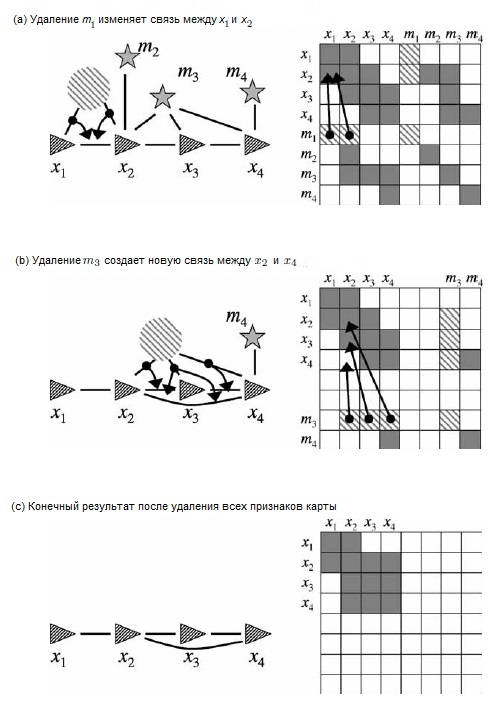
\includegraphics[width=1
	\linewidth]{113orig}}
	\caption{ ( Рис. 11.3 Уменьшение графа в GraphSLAM:   для выделения связей, дуги, соединяющих только положения робота, удалены.)}
	\label{fig:113orig}
\end{figure}

Красота такого подхода состоит в возможности постепенно разбивать задачу связности на более мелкие. Удаляя каждый признак $m_j$ из $\varOmega$ и $\xi$, постепенно можно прийти к значительно меньшему информационному представлению $\bar{\varOmega}$ и $\bar{\xi}$, определённому только по пути робота. Это уменьшение может быть выполнено за время, линейно зависящее от размера карты. Тем самым выполняется обобщение метода уничтожения переменной для инверсии матрицы информационного представления, в котором также поддерживается информационное состояние. Апостериорное распределение по пути робота теперь можно восстановить, как $\bar{\varSigma}=\bar{\varOmega}^{-1}$ и $\bar{\mu}=\bar{\varSigma}\xi$.  К сожалению, такт уменьшения размера не уничтожает циклы в апостериорном распределении. Оставшаяся задача математического вывода может потребовать дополнительных нелинейных шагов.

На последнем шаге GraphSLAM восстанавливает расположение признаков. Теоретически, это достигается построением новой информационной матрицы $\varOmega_j$ и информационного вектора $\xi_j$ для каждого признака $m_j$. Они определены для переменной признака $m_j$ и положений $\tau(j)$, в которых он наблюдался. Матрица содержит начальные связи между $m_j$ и $\tau(j)$, но положения $\tau(j)$ установлены в значения $\bar{\mu}$, без учёта неопределённости. С информационной точки зрения, достаточно просто вычислить местоположение $m_j$, используя общий метод обращения матриц. Ясно, что $\varOmega_j$ содержит только элементы, соединяющие признак $m_j$, поэтому обращение займёт время, линейно зависящее от $\tau(j)$.

Должно быть очевидно, почему выражение в виде графа столь естественно. Полная задача SLAM решается локальным добавлением информации в большой информационный граф по одному ребру за такт для каждого измерения $z_t^i$ и каждого управляющего воздействия $u_t$. Чтобы превратить такую информацию в оценку карты и пути робота, она сначала подвергается линеаризации, а затем информация между положениями и признаками последовательно смещается в информацию между парами положений. Результирующая структура состоит только из положений робота, которые вычисляются, используя инверсию матриц. После восстановления положений местоположения признаков вычисляются одно за другим, на основе начальной информации отношения признака к положению.\\

\textbf{11.3	Алгоритм GraphSLAM}\\

Давайте выполним точное вычисление различных тактов алгоритма GraphSLAM. \textit{Алгоритм полного GraphSLAM }будет описан в виде последовательности шагов. Главной трудностью реализации простого аддитивного информационного алгоритма является преобразование условной вероятности вида $p(z_t^i|x_t,m)$ и $p(x_t|u_t,x_{t-1})$ в связь в информационной матрице. Все элементы информационной матрицы линейны, поэтому этот шаг включает линеаризацию $p(z_t^i|x_t,m)$ и $p(x_t|u_t,x_{t-1})$. В EKF SLAM эта линеаризация была вычислена с помощью якобиана для средних оценок положений $\mu_{0:t}$. Для построения начальной информационной матрицы $\varOmega$ и $\xi$ требуется начальная оценка $\mu_{0:t}$ для всех положений $x_{0:t}$. 

\begin{table}[H]
\begin{center}
\begin{tabular}{|l|}
\hline
{}\\
1: \textbf{Algorithm GraphSLAM\_initialize}$(u_{1:t}):\qquad\qquad\qquad\qquad$ \\
2:\hspace{5mm}
\begin{minipage}{0.2\textwidth}
				\begin{equation*}
				\left(\begin{array}{c}
				\mu_{0,x}\\
				\mu_{0,y}\\
				
\mu_{0,\theta}\\
				\end{array}\right)
=
\left(\begin{array}{c}
0\\
0\\

0\\
\end{array}\right)				\end{equation*}
\end{minipage}\\
3:\hspace{5mm}$\textit{for all controls}\,\,u_t=(v_t\,\,\omega_t)^T\,\,\textit{do}$\\
4:\hspace{10mm}
\begin{minipage}{0.2\textwidth}
				\begin{equation*}
				\left(\begin{array}{c}
				\mu_{t,x}\\
				\mu_{t,y}\\
				
\mu_{t,\theta}
				\end{array}\right)
=
\left(\begin{array}{c}
\mu_{t-1,x}\\
\mu_{t-1,y}\\

\mu_{t-1,\theta}
\end{array}\right)				\end{equation*}
\end{minipage}\\
4:\hspace{15mm}
\begin{minipage}{0.2\textwidth}
				\begin{equation*}
				+
				\left(\begin{array}{c}
				-\frac{v_t}{\omega_t}\sin\mu_{t-1,\theta}+\frac{v_t}{\omega_t}\sin(\mu_{t-1,\theta}+\omega_t\varDelta t)\\
				\frac{v_t}{\omega_t}\cos\mu_{t-1,\theta}-\frac{v_t}{\omega_t}\cos(\mu_{t-1,\theta}+\omega_t\varDelta t)\\
				\omega_t\varDelta t\\
				\end{array}\right)
				\end{equation*}
\end{minipage}\\
5:\hspace{5mm}$\textit{endfor}$\\
6:\hspace{5mm}$\textit{return}\,\,\mu_{0:t}$\\

{}\\
\hline
\end{tabular}
\caption{(Таблица 11.1  Инициализация вектора среднего положения $\mu_{1:t}$ в алгоритме GraphSLAM.)}
\end{center}
\end{table}

\begin{table}[H]
\begin{center}
\begin{tabular}{|l|}
\hline
{}\\
1:\textbf{ Algorithm GraphSLAM\_linearize}$(u_{1:t},z_{1:t},c_{1:t},\mu_{0:t}):\qquad\qquad$ \\
2:\hspace{5mm}$\textit{set}\,\,\varOmega=0,\,\xi=0$\\
3:\hspace{5mm}
\begin{minipage}{0.2\textwidth}
				\begin{equation*}
\textit{add}	\left(\begin{array}{ccc}
\infty&0&0\\
0&\infty&0\\
0&0&\infty\\
\end{array}\right)
\,\,\textit{to}\,\,\varOmega\,\,\textit{at}\,\,x_0				\end{equation*}
\end{minipage}\\
4:\hspace{5mm}$\textit{for all controls}\,\,u_t=(v_t\,\,\omega_t)^T\,\,\textit{do}$\\
5:\hspace{10mm}
\begin{minipage}{0.2\textwidth}
\begin{equation*}
\hat{x}_t=\mu_{t-1}+
\left(\begin{array}{c}
-\frac{v_t}{\omega_t}\sin\mu_{t-1,\theta}+\frac{v_t}{\omega_t}\sin(\mu_{t-1,\theta}+\omega_t\varDelta t)\\
\frac{v_t}{\omega_t}\cos\mu_{t-1,\theta}-\frac{v_t}{\omega_t}\cos(\mu_{t-1,\theta}+\omega_t\varDelta t)\\
\omega_t\varDelta t\\
\end{array}\right)				\end{equation*}
\end{minipage}\\
6:\hspace{10mm}
\begin{minipage}{0.2\textwidth}
\begin{equation*}
G_t=
\left(\begin{array}{ccc}
				1&0&-\frac{v_t}{\omega_t}\cos\mu_{t-1,\theta}+\frac{v_t}{\omega_t}\cos(\mu_{t-1,\theta}+\omega_t\varDelta t)\\
				0&1&-\frac{v_t}{\omega_t}\sin\mu_{t-1,\theta}+\frac{v_t}{\omega_t}\sin(\mu_{t-1,\theta}+\omega_t\varDelta t)\\
				0&0&1\\
				\end{array}\right)
				\end{equation*}
\end{minipage}\\
{}\\
\hspace{35mm}$\boxed{\textit{продолжение на следующей странице}}$\\

\hline
\end{tabular}
\end{center}
\end{table}

\begin{table}[H]
\begin{center}
\begin{tabular}{|l|}
\hline
\hspace{50mm}$\boxed{\textit{начало на предыдущей странице}}$\\
{}\\
7:\hspace{10mm}
\begin{minipage}{0.2\textwidth}
\begin{equation*}
\textit{add}	\left(\begin{array}{c}
-G_t^T\\
1\\
\end{array}\right)
\,\,R_t^{-1}\,(-G_t\,\,\,1)\textit{to}\,\,\varOmega\,\,\textit{at}\,\,x_t\,\,\textit{and}\,\,x_{t-1}			\end{equation*}
\end{minipage}\\
8:\hspace{10mm}
\begin{minipage}{0.2\textwidth}
\begin{equation*}
\textit{add}	\left(\begin{array}{c}
-G_t^T\\
1\\
\end{array}\right)
\,\,R_t^{-1}\,[\hat{x}_t-G_t\,\mu_{t-1}]\textit{to}\,\,\xi\,\,\textit{at}\,\,x_t\,\,\textit{and}\,\,x_{t-1}		\end{equation*}
\end{minipage}\\
9:\hspace{6mm}$\textit{endfor}$\\
10:\hspace{4mm}$\textit{для всех измерений}\,\,z_t\,\,\textit{do}$\\
11:\hspace{4mm}
\begin{minipage}{0.2\textwidth}
\begin{equation*}
Q_t=	\left(\begin{array}{ccc}
\sigma_r^2&0&0\\
0&\sigma_\phi^2&0\\
0&0&\sigma_s^2\\
\end{array}\right)
\end{equation*}
\end{minipage}\\
12:\hspace{9mm}$\textit{для всех наблюдаемых признаков}\,\,z_t^i=(r_t^i\,\,\phi_t^i\,\,s_t^i)^T\,\,\textit{do}$\\
13:\hspace{14mm}$j=c_t^i$\\
14:\hspace{14mm}
\begin{minipage}{0.2\textwidth}
\begin{equation*}
\delta=\left(\begin{array}{c} \delta_x\\
\delta_y\\
\end{array} \right)\\
=\left(\begin{array}{c} \mu_{j,x}-\mu_{t,x}\\
\mu_{j,y}-\mu_{t,y}\\
\end{array} \right)\\
\end{equation*}
\end{minipage}\\
15:\hspace{14mm}$q=\delta^T\,\delta$\\
16:\hspace{14mm}
\begin{minipage}{0.2\textwidth}
\begin{equation*}
\hat{z}_t^i=\left(\begin{array}{c} \sqrt{q}\\
\text{atan2}(\delta_y,\delta_x)-\mu_{t,\theta}\\
s_j
\end{array} \right)\\
\end{equation*}
\end{minipage}\\
17:\hspace{9mm}
\begin{minipage}{0.2\textwidth}
\begin{equation*}
H_t^i=\frac{1}{q}\,\left(\begin{array}{cccccc} -\sqrt{q}\delta_x&-\sqrt{q}\delta_y&0&+\sqrt{q}\delta_x&\sqrt{q}\delta_y&0\\
\delta_y&-\delta_x&-q&-\delta_y&+\delta_x&0\\
0&0&0&0&0&q
\end{array} \right)\\
\end{equation*}
\end{minipage}\\
18:\hspace{14mm}
$\textit{добавить}	
\,\,H_t^{iT}\,Q_t^{-1}\,H_t^i\,\,\textit{к}\,\,\varOmega\,\,\textit{в}\,\,x_t\,\,\textit{и}\,\,m_j$\\		19:\hspace{14mm}
\begin{minipage}{0.2\textwidth}
\begin{equation*}
\textit{добавить}\,\,H_t^{iT}\,Q_t^{-1}\,[z_t^i-\hat{z}_t^i+H_t^i
\left(\begin{array}{c}
\mu_{t,x}\\\mu_{t,y}\\\mu_{t,\theta}\\\mu_{j,x}\\\mu_{j,y}\\\mu_{j,s}\\
\end{array}\right)]
\,\,\textit{к}\,\,\xi\,\,\textit{в}\,\,x_t\,\,\textit{и}\,\,m_j				\end{equation*}
\end{minipage}\\20:\hspace{9mm}$\textit{endfor}$\\	
21:\hspace{4mm}$\textit{endfor}$\\
22:\hspace{4mm}$\textit{return}\,\,\varOmega,\xi$\\
{}\\
\hline
\end{tabular}
\caption{(Таблица 11.2    Вычисление $\varOmega$ и $\xi$ в GraphSLAM.)}
\end{center}
\end{table}

\begin{table}[H]
\begin{center}
\begin{tabular}{|l|}
\hline
{}\\
1: \textbf{Algorithm GraphSLAM\_reduce}$(\varOmega,\xi):\qquad\qquad\qquad\qquad$ \\
{}\\
2:\hspace{5mm}$\bar{\varOmega}=\varOmega$\\
3:\hspace{5mm}$\bar{\xi}=\xi$\\
4:\hspace{5mm}$\textit{для каждого признака\,\,j\,\,do}$\\
5:\hspace{10mm}$\textit{пусть}\,\,\tau(j)\,\,\textit{набор всех положений}\,\,x_t\,\,\textit{в которых наблюдался j}$\\
6:\hspace{10mm}$\textit{вычесть}\,\,\bar{\varOmega}_{\tau(j),j}\bar{\varOmega}_{j,j}^{-1}\xi_j\,\,\textit{из}\,\,\bar{\xi}\,\,\textit{at}\,\,x_{\tau(j)}\,\,\textit{and}\,\,m_j$\\
7:\hspace{10mm}$\textit{вычесть}\,\,\bar{\varOmega}_{\tau(j),j}\bar{\varOmega}_{j,j}^{-1}\bar{\varOmega}_{j,\tau(j)}\,\,\textit{из}\,\,\bar{\varOmega}\,\,\textit{в}\,\,x_{\tau(j)}\,\,\textit{и}\,\,m_j$\\
8:\hspace{10mm}$\textit{удалить из}\,\,\bar{\varOmega}\,\,\textit{и}\,\,\bar{\xi}\,\,\textit{все строки/столбцы, соответсвующие j}$\\
9:\hspace{5mm}$\textit{endfor}$\\
10:\hspace{4mm}$\textit{return}\,\,\bar{\varOmega},\bar{\xi}$\\
{}\\
\hline
\end{tabular}
\caption{(Таблица 11.3 Алгоритм уменьшения размера информационного представления апостериорного распределения в GraphSLAM.)}
\end{center}
\end{table}

\begin{table}[H]
\begin{center}
\begin{tabular}{|l|}
\hline
{}\\
1: \textbf{Algorithm GraphSLAM\_solve}$(\bar{\varOmega},\bar{\xi},\varOmega,\xi):\qquad\qquad\qquad\qquad$ \\
{}\\
2:\hspace{5mm}$\varSigma_{0:t}=\bar{\varOmega}^{-1}$\\
3:\hspace{5mm}$\mu_{0:t}=\varSigma_{0:t}\bar{\xi}$\\
4:\hspace{5mm}$\textit{для каждого признака\,\,j\,\,do}$\\
5:\hspace{10mm}$\textit{set}\,\,\tau(j)\,\,\textit{к набору всех положений}\,\,x_t\,\,\textit{в которых наблюдался j}$\\
6:\hspace{10mm}$\mu_j=\varOmega_{j,j}^{-1}(\xi_j+\varOmega_{j,\tau(j)}\bar{\mu}_{\tau(j)})$\\
7:\hspace{5mm}$\textit{endfor}$\\
8:\hspace{5mm}$\textit{return}\,\,\mu,\varSigma_{0:t}$\\
{}\\
\hline
\end{tabular}
\caption{(Таблица 11.4    Алгоритм обновления апостериорного распределения $\mu$.)}
\end{center}
\end{table}

\begin{table}[H]
\begin{center}
\begin{tabular}{|l|}
\hline
{}\\
1: \textbf{Algorithm GraphSLAM\_known\_correspondence}$(u_{1:t},z_{1:t},c_{1:t}):\qquad$ \\
{}\\
2:\hspace{5mm}$\mu_{0:t}=\textbf{GraphSLAM\_initialize}\,(u_{1:t})$\\
3:\hspace{5mm}$\textit{повторять}$\\
4:\hspace{10mm}$\varOmega,\xi=\textbf{GraphSLAM\_linearize}\,(u_{1:t},z_{1:t},c_{1:t}\mu_{0:t})$\\
5:\hspace{10mm}$\bar{\varOmega},\bar{\xi}=\textbf{GraphSLAM\_reduce}\,(\varOmega,\xi)$\\
6:\hspace{10mm}$\mu,\varSigma_{0:t}=\textbf{GraphSLAM\_solve}\,(\bar{\varOmega},\bar{\xi},\varOmega,\xi)$\\
7:\hspace{5mm}$\textit{до сходимости}$\\
8:\hspace{5mm}$\textit{return}\,\,\mu$\\
{}\\
\hline
\end{tabular}
\caption{(Таблица 11.5 Алгоритм GraphSLAM для полной задачи SLAM с известным соответствием.)}
\end{center}
\end{table}

Существует большое количество решений задачи нахождения начального среднего $\mu$, подходящего для линеаризации. Например, можно запустить алгоритм EKF SLAM и использовать его оценку для линеаризации. В этой главе будет использован ещё более простой приём. Начальная оценка будет получена простым связываем воедино модели движения $p(x_t|u_t,x_{t-1})$.Такой алгоритм приводится в Таблице 11.1, и называется \textbf{GraphSLAM\_initialize}. Этот алгоритм принимает на вход сигналы управления $u_{1:t}$ и выдаёт на выход последовательность оценок положений $\mu_{0:t}$. В нем первое положение инициализируется нулём, а затем последующие положения вычисляются путём рекурсивного применения модели движения на основе скорости. Поскольку нас интересует только средний вектор положений $\mu_{0:t}$,в алгоритме \textbf{GraphSLAM\_initialize} используется только детерминированная часть модели движения. Измерения в оценке также не учитываются.

Когда начальное значение $\mu_{0:t}$ доступно, алгоритм GraphSLAM создаёт полную информационную матрицу SLAM $\varOmega$ и соответствующий информационный вектор $\xi$, выполняя линеаризацию всех связей на графе. Алгоритм \textbf{GraphSLAM\_linearize} приведён в Таблице 11.2. В нём присутствует множество математических выражений, смысл которых будет раскрыт ниже в разделе математического вывода алгоритма. \textbf{GraphSLAM\_linearize} принимает на вход набор управляющих сигналов, $u_{1:t}$, измерения $z_{1:t}$, связанные переменные соответствия $c_{1:t}$ и средние оценки положения $\mu_{0:t}$. Затем с помощью линеаризации постепенно создаётся информационная матрица $\varOmega$ и информационный вектор $\xi$, локально добавляя субматрицы в соответствии с информацией, полученной из каждого измерения и каждого управляющего воздействия.

В частности, в строке 2 в \textbf{GraphSLAM\_linearize} выполняется инициализация информационных элементов. «Бесконечный» информационный элемент в строке 3 фиксирует начальное положение $x_0$ по координатам $(0\,\,0\,\,0)^T$ . Это необходимо, поскольку в противном случае результирующая матрица становится вырожденной, отражая факт невозможности восстановления абсолютных оценок на основании только относительной информации.

Управление интегрируется в строках с 4 по 9 алгоритма \textbf{GraphSLAM\_linearize}. Положение $\hat{x}$ и якобиан $G_t$, вычисленные в строках 5 и 6, отображают линейную аппроксимацию нелинейной функции управления $g$. Как очевидно следует из этих уравнений, такт линеаризации использует оценки положения $\mu_{0:t-1}$ при $\mu_0=(0\,\,0\,\,0)^T$ . Это ведёт к обновлениям $\varOmega$ и $\xi$, вычисленных в строках 7 и 8, соответственно. Оба члена добавляются в соответствующие строки и столбцы $\varOmega$ и $\xi$.  Это добавление реализует включение нового ограничения в апостериорную оценку SLAM, что очень близко к интуитивному описанию в предыдущем разделе.

Измерения интегрируются в строках с 10 по 21 \textbf{Graph- SLAM\_linearize}. Матрица $Q_t$, вычисленная в строке 11, представляет собой уже знакомую ковариацию шумов измерений. В строках с 13 по 17 выполняется разложение в ряд Тейлора функции измерений, определённой здесь для модели измерения на основе признаков, которая была описана в разделе 6.6. Следует обратить внимание на реализацию в строке 16, поскольку угловые величины могут быть произвольно смещены на $2\pi$. Это вычисление даёт операцию обновления измерения в строках 18 и 19. Матрица, добавляемая к $\varOmega$ в строке 18, имеет размер $6\times6$. Для добавления она разбивается на матрицу размером $3\times3$ для положения $x_t$, матрицу размером $3\times3$ для признака $m_j$, и две матрицы размером $3\times3$ каждая для связей между $x_t$ и $m_j$. Они добавляются к $\varOmega$ в соответствующих строках и столбцах. Аналогично, вектор добавляется к информационному вектору $\xi$ размером 5 по вертикали. Он также разбивается на векторы размером 3 и 2 и добавляется к элементам, соответствующим $x_t$ и $m_j$. Результатом работы \textbf{GraphSLAM\_linearize} являются информационный вектор $\xi$ и матрица $\varOmega$. Уже было отмечено, что $\varOmega$ является разреженной матрицей. Она содержит ненулевые субматрицы только вдоль главной диагонали, между последовательными положениями, и между положениями и признаками на карте. Время работы алгоритма линейно зависит от $t$, количества тактов времени, когда были получены данные.

Следующим шагом алгоритма GraphSLAM является уменьшение размерности информационной матрицы и вектора. Это достигается с помощью алгоритма \textbf{GraphSLAM\_reduce} в Таблице 11.3. Этот алгоритм принимает на вход $\varOmega$ и $\xi$, определённые по всему пространству признаков карты и положений, а на выход поступает уменьшенная матрица $\bar{\varOmega}$ и векторы $\bar{\xi}$, определённые в пространстве всех положений, но без карты! Это преобразование выполняется последовательным удалением признаков $m_j$, в строках с 4 по 9 \textbf{GraphSLAM\_reduce}. Учёт точных индексов каждого элемента $\bar{\varOmega}$  и $\bar{\xi}$ достаточно утомителен, поэтому в Таблице 11.3 приводится лишь общее описание.

В строке 5 вычисляется набор положений $\tau(j)$, в которых робот наблюдает признак $j$.  Затем  из существующих матриц $\bar{\varOmega}:\bar{\varOmega}_{j,j}$ и $\bar{\varOmega}_{\tau(j),j}$ извлекаются две субматрицы.  $\bar{\varOmega}_{j,j}$ это квадратная субматрица между $m_j$  и $m_j$, а $\bar{\varOmega}_{\tau(j),j}$  составлена из недиагональных элементов между $m_j$ и переменными положения $\tau(j)$. Затем из информационного вектора состояний $\bar{\xi}$ извлекаются элементы, соответствующие $j$-му признаку, обозначаемому здесь как $\xi_j.$ Затем из $\bar{\varOmega}$ и $\bar{\xi}$ вычитается информация, как показано в строках 6 и 7. После этой операции строки и столбцы для признака $m_j$ становятся равны нулю. Эти строки и столбцы удаляются, что уменьшает размер $\bar{\varOmega}$  и $\bar{\xi}$, соответственно.  Процесс повторяется до удаления всех признаков, пока в $\bar{\varOmega}$ и $\bar{\xi}$  не останутся только положения. Сложность \textbf{GraphSLAM\_reduce} снова линейно зависит от $t$.

Последним шагом в алгоритме GraphSLAM является вычисление математического ожидания и ковариации для всех положений на пути робота, и средней оценки местоположения для всех признаков на карте. Это достигается с помощью алгоритма \textbf{GraphSLAM\_solve}, приведённого в Таблице 11.4. В строках 2 и 3 вычисляются оценки пути $\mu_{0:t}$ с помощью инверсии уменьшенной информационной матрицы $\bar{\varOmega}$ и умножения результирующей ковариации на информационный вектор. Затем в \textbf{GraphSLAM\_solve} в строках с 4 по 7 вычисляется местоположение каждого признака. Возвращаемое значение \textbf{GraphSLAM\_solve} содержит средний путь робота и все признаки карты, но только ковариацию для пути робота. Было замечено, что существуют другие, более эффективные способы вычисления $\mu_{0:t}$, не требующие обращения матрицы. Они будут обсуждаться ближе к концу главы, в описании применения стандартных методов оптимизации для GraphSLAM.

Качество решения, вычисленного алгоритмом GraphSLAM, зависит от качества начальных средних оценок, вычисленных \textbf{GraphSLAM\_initialize}. Компоненты координат $x$- и $y$- этих оценок линейно воздействуют на соответствующие модели, поэтому линеаризация от них никак не зависит. Но для переменных ориентации $\mu_{0:t}$ это не так. Ошибки в начальных оценках влияют на точность приближения разложением в ряд Тейлора, что, в свою очередь, влияет на результат.

Для уменьшения потенциальных ошибок разложения в ряд Тейлора при линеаризации, процедуры \textbf{GraphSLAM\_linearize}, \textbf{GraphSLAM\_reduce}, и \textbf{GraphSLAM\_solve} могут запускаться несколько раз подряд на одном и том же наборе данных. Каждая итерация принимает на вход оценочный вектор $\mu_{0:t}$ предыдущей итерации, выдавая новую, уточнённую оценку. Повторение итераций GraphSLAM необходимо только когда начальные оценки положения имеют большую ошибку (более 20 градусов по углу ориентации). Небольшого количества итераций (обычно, трёх) достаточно.

В Таблице 11.5 приводится общий вид алгоритма. В нем инициализируются средние значения, затем повторяется такты создания матрицы, уменьшения размерности, и решения. Обычно, для сходимости достаточно двух-трёх итераций. Результирующее среднее $\mu$ является наилучшей гипотезой для пути робота и карты.\\

\textbf{11.4	Математический вывод GraphSLAM}\\

Вывод алгоритма GraphSLAM начинается с вывода рекурсивной формулы для вычисления полного апостериорного распределения SLAM, выраженного в информационном виде. Затем будет подробно описан каждый член этого распределения, а затем выведен аддитивный шаг обновления SLAM с помощью разложения в ряд Тейлора. После этого будут выведены необходимые уравнения для восстановления пройденного пути и карты.\\

\textbf{11.4.1	Полное апостериорное распределение SLAM}\\

Также, как и при обсуждении EKF SLAM, будет выгодно ввести переменную для дополненного состояния в полной проблеме SLAM. Будем использовать $y$ для обозначения переменных состояния, сочетающих одно или более положений $x$ на карте $m$. В частности, определим $y_{0:t}$ в виде вектора, состоящего из пути $x_{0:t}$ и карты $m$, где $y_t$ состоит из моментального положения в момент времени $t$ и карты $m$:\\

(11.4)
\begin{minipage}{0.2\textwidth}
\begin{equation*}
y_{0:t}=\,\left(\begin{array}{c}x_0\\
x_1\\
\vdots\\
x_t\\
m
\end{array} \right)\\\qquad
\text{и}\qquad
y_t=\,\left(\begin{array}{c}
x_t\\
m\end{array} \right)
\end{equation*}
\end{minipage}

Апостериорное распределение для полной задачи SLAM $p(y_{0:t}|z_{1:t},u_{1:t},c_{1:t})$, где $z_{1:t}$  - измерения с соответствиями $c_{1:t}$, а $u_{1:t}$ – управляющие воздействия. Теорема Байеса позволяет выполнить факторизацию этого распределение:\\

(11.5) 
\begin{equation*}
\begin{split}
p(y_{0:t}&|z_{1:t},u_{1:t},c_{1:t})\\
&=\eta\,p(z_t|y_{0:t},z_{1:t-1},u_{1:t},c_{1:t})p(y_{0:t}|z_{1:t-1},u_{1:t},c_{1:t})
\end{split}
\end{equation*}

где $\eta$ – уже знакомый нормализующий член. Первое значение  вероятности с правой стороны может быть упрощено отбрасыванием нерелевантных переменных:\\

(11.6)
$$p(z_t|y_{0:t},z_{1:t-1},u_{1:t},c_{1:t})=p(z_t|y_t,c_t)$$

похожим образом можно факторизовать вторую вероятность, разбив $y_{0:t}$ по $x_t$ и $y_{0:t-1}$, что даёт\\

(11.7)
\begin{equation*}
\begin{split}
p(y_{0:t}&|z_{1:t-1},u_{1:t},c_{1:t})\\
&=p(x_t|y_{0:t-1},z_{1:t-1},u_{1:t},c_{1:t})p(y_{0:t-1}|z_{1:t-1},u_{1:t},c_{1:t})\\
&=p(x_t|x_{t-1},u_t)p(y_{0:t-1}|z_{1:t-1},u_{1:t-1},c_{1:t-1})
\end{split}
\end{equation*}

Вставка этих выражений обратно в (11.5) даст рекурсивное определение полного апостериорного распределения SLAM:\\

(11.8)
\begin{equation*}
\begin{split}
p(y_{0:t}&|z_{1:t},u_{1:t},c_{1:t})\\
&=\eta\,p(z_t|y_t,c_t)p(x_t|x_{t-1},u_t)p(y_{0:t-1}|z_{1:t-1},u_{1:t-1},c_{1:t-1})\\
\end{split}
\end{equation*}

Выражение в закрытом виде получается с помощью индукции по $t$. Здесь $p(y_0)$ - априорная вероятность по карте $m$ и начальному положению $x_0$.\\

(11.9)
\begin{equation*}
\begin{split}
p(y_{0:t}|z_{1:t},u_{1:t},c_{1:t})&=\eta\,p(y_0)\prod_t p(x_t|x_{t-1},u_t)p(z_t|y_t,c_t)\\
&=\eta\,p(y_0)\prod_t\left[  p(x_t|x_{t-1},u_t)\prod_i p(z_t^i|y_t,c_t^i)\right] 
\end{split}
\end{equation*}

Здесь, как и прежде, $z_t^i$ это $i$-е измерение в векторе измерения $z_t$ в момент времени $t$. Априорная вероятность $p(y_0)$ разбивается на две независимые априорные вероятности, $p(x_0)$ и $p(m)$. В SLAM обычно нет никаких предварительных данных о карте $m$, поэтому $p(y_0)$ просто заменяется $p(x_0)$, а множитель $p(m)$ выносится в нормализующий член $\eta$.\\

\textbf{11.4.2	Отрицательный логарифм апостериорной вероятности}\\

В информационном виде вероятности представлены логарифмическими выражениями. Форма апостериорной вероятности log-SLAM напрямую следует из предыдущего равенства:\\

(11.10)
\begin{equation*}
\begin{split}
\log\,p(y_{0:t}&|z_{1:t},u_{1:t},c_{1:t})\\
&=\text{const.}+\log p(x_0)+\sum_t\left[ \log p(x_t|x_{t-1},u_t)+\sum_i\log p(z_t^i|y_t,c_t^i)\right] 
\end{split}
\end{equation*}

Так же, как в Главе 10, допустим, что результат движения робота нормально распределён по $\mathcal{N}(g(u_t, x_{t-1}), R_t)$, где $g$ – детерминированная функция движения, а $R_t$ – ковариация ошибки движения. Аналогично, измерения $z_t^i$ генерируются согласно распределению $\mathcal{N}(h(y_t,c_t^i),Q_t)$, где $h$ уже знакомая функция измерения, а $Q_t$ – ковариация ошибки измерения. В виде уравнений получается\\

(11.11)
$$p(x_t|x_{t-1},u_t)=\eta\,\exp\left\lbrace -\frac{1}{2}(x_t-g(u_t,x_{t-1}))^TR_t^{-1}(x_t-g(u_t,x_{t-1}))\right\rbrace $$

(11.12)
$$p(z_t^i|y_t,c_t^i)=\eta\,\exp\left\lbrace -\frac{1}{2}(z_t^i-h(y_t,c_t^i))^TQ_t^{-1}(z_t^i-h(y_t,c_t^i))\right\rbrace $$

Априорная вероятность $p(x_0)$ в (11.10) также выражена распределением, похожим на гауссовское. Она связывает начальное положение $x_0$ и началу глобальной системы координат:  $x_0=(0\,\,0\,\,0)^T$:\\

(11.13)
$$p(x_0)=\eta\,\exp\left\lbrace -\frac{1}{2}x_0^T\,\varOmega_0\,x_0\right\rbrace $$
с\\

(11.14)
\begin{minipage}{0.2\textwidth}
\begin{equation*}
\varOmega_0=\,\left(\begin{array}{ccc}\\
\infty&0&0\\
0&\infty&0\\
0&0&\infty\\
\end{array} \right)
\end{equation*}
\end{minipage}

Сейчас не нужно беспокоиться о том, что значение $\infty$ невозможно представить, поскольку его можно легко заменить достаточно большим положительным числом. Это даст следующую квадратичную форму отрицательной log-SLAM апостериорной вероятности в (11.10):\\

(11.15)
\begin{multline*}
-\log\,p(y_{0:t}|z_{1:t},u_{1:t},c_{1:t})\\
=\text{const.}+\frac{1}{2}[  x_0^T\varOmega_0x_0+\sum_t(x_t-g(u_t,x_{t-1}))^TR_t^{-1}(x_t-g(u_t,x_{t-1})) \\
+ \sum_t\sum_i(z_t^i-h(y_t,c_t^i))^TQ_t^{-1}(z_t^i-h(y_t,c_t^i))]  
\end{multline*}

В основном, это то же самое, что $J_{GraphSLAM}$ в выражении (11.3), с некоторыми различиями в силу отбрасывания нормализующих постоянных (включая умножение на -1). Выражение (11.15) показывает важную характеристику полной апостериорной вероятности SLAM в информационном виде: она состоит из определённого числа квадратичных членов, одного для априорной вероятности, и по одному для каждого управляющего воздействия и измерения.\\

\textbf{11.4.3	Разложение в ряд Тейлора}\\

Различные члены в Выражении (11.15) квадратичны для функций $g$ и $h$, но не для переменных, которые следует оценить (положения и карта).\\
ЛИНЕАРИЗАЦИЯ\\
GraphSLAM решает проблему линеаризации $g$ и $h$ разложением в ряд Тейлора, то есть полностью аналогично выражениям (10.14) и (10.18) в выводе EKF. В частности, получается:\\

(11.16)
$$g(u_t,x_{t-1})\approx g(u_t,\mu_{t-1})+G_t(x_{t-1}-\mu_{t-1})$$

(11.17)
$$h(y_t,c_t^i)\approx h(\mu_t,c_t^i)+H_t^i(y_t-\mu_t)$$

Здесь $\mu_t$ - текущая оценка вектора состояний $y_t$, а $H_t^i=h_t^i\,F_{x,j}$ как было определено в выражении (10.19).

Это линейное приближение превращает логарифм правдоподобия (11.15) в функцию, квадратичную по $y_{0:t}$. В частности,получается\\

(11.18)
\begin{equation*}
\begin{split}
\log\,p(y_{0:t}&|z_{1:t},u_{1:t},c_{1:t})=\text{const.}-\frac{1}{2}\\
&\{x_0^T\varOmega_0x_0+\sum_t[x_t-g(u_t,\mu_{t-1})-G_t(x_{t-1}-\mu_{t-1})]^T\\
&R_t^{-1}[x_t-g(u_t,\mu_{t-1})-G_t(x_{t-1}-\mu_{t-1})]\\
&+\sum_i [z_t^i-h(\mu_t,c_t^i)-H_t^i(y_t-\mu_t)]^TQ_t^{-1}[z_t^i-h(\mu_t,c_t^i)-H_t^i(y_t-\mu_t)]\} 
\end{split}
\end{equation*}

Эта функция действительно квадратична по $y_{0:t}$, и необходимо перегруппировать члены, отбросив несколько констант.\\

(11.19)
$$\log\,p(y_{0:t}|z_{1:t},u_{1:t},c_{1:t})=\text{const.}$$
$$-\frac{1}{2}\underbrace{x_0^T\varOmega_0x_0}_{\text{квадратична по}\,x_0}-\frac{1}{2}\sum_t\underbrace{{x_{t-1:t}^T}
\left(\begin{array}{c}-G_t^T\\
1\\
\end{array} \right)R_t^{-1}(-G_t\,\,1)x_{t-1:t}}_{\text{квадратична по}\,x_{t-1:t}}$$
$$+\underbrace {x_{t-1:t}^T\left(\begin{array}{c}-G_t^T\\
1\\
\end{array} \right)R_t^{-1}[g(u_t,\mu_{t-1})-G_t\mu_{t-1}]}_{\text{линейна в}\,x_{t-1:t}}$$
$$-\frac{1}{2}\sum_i\underbrace{y_t^TH_t^{iT}Q_t^{-1}H_t^iy_t}_{\text{квадратична по}\,y_t}+\underbrace{y_t^TH_t^{iT}Q_t^{-1}[z_t^i-h(\mu_t,c_t^i)+H_t^i\mu_t]}_{\text{линейна в}\,y_t}$$

Здесь $x_{t-1:t}$ определяет вектор состояния, присоединяя $x_{t-1}$ и $x_t$. Отсюда можно записать $(x_t-G_t\,\,x_{t-1})^T=x_{t-1:t}^T(-G_t\,\,1)^T=x_{t-1:t}^T\left(\begin{array}{c}-G_t^T\\
1\\
\end{array} \right)$.

если собрать все квадратичные члены в матрицу $\varOmega$, а все линейные – в вектор $\xi$, можно увидеть, что выражение (11.19) имеет вид\\

(11.20)
$$\log\,p(y_{0:t}|z_{1:t},u_{1:t},c_{1:t})=\text{const.}-\frac{1}{2}y_{0:t}^T\varOmega y_{0:t}+y_{0:t}^T \xi$$

\textbf{11.4.4	Создание информационного представления}\\

Эти элементы можно напрямую взять из (11.19), и убедиться, что они действительно реализуют алгоритм \textbf{GraphSLAM\_linearize} в Таблице 11.2:\\

•	Априорная вероятность. Начальное положение показано квадратичным членом $\varOmega_0$ по переменной начального положения $x_0$ в информационной матрице. Допуская соответствующее расширение матрицы $\varOmega_0$ до размерности $y_{0:t}$, получим\\

(11.21)
$$\varOmega\,\,\longleftarrow\,\,\varOmega_0$$

Эта инициализация выполняется в строках 2 и 3 алгоритма \textbf{GraphSLAM\_linearize}.\\

•	\textbf{Управление.} Из (11.19), можно увидеть, что каждое управляющее воздействие $u_t$ добавляет к $\varOmega$ и $\xi$ следующие члены, при условии, что матрицы расширены до одинаковых размеров:\\

(11.22)
$$\varOmega\,\,\longleftarrow\,\,\varOmega+\left(\begin{array}{c}-G_t^T\\
1\\
\end{array} \right)R_t^{-1}(-G_t\,\,1)$$

(11.23)
$$\xi\,\,\longleftarrow\,\,\xi+\left(\begin{array}{c}-G_t^T\\
1\\
\end{array} \right)R_t^{-1}[g(u_t,\mu_{t-1})-G_t \mu_{t-1}]$$

Это выполняется в строках с 4 по 9 в \textbf{GraphSLAM\_linearize}.\\

•	\textbf{Измерения.} Согласно Выражению (11.19), каждое измерение $z_t^i$ преобразует $\varOmega$ и $\xi$ добавлением следующих членов, снова подразумевая расширение матриц до одинаковых размеров:\\

(11.24)
$$\varOmega\,\,\longleftarrow\,\,\varOmega+H_t^{iT}Q_t^{-1}H_t^i$$

(11.25)
$$\xi\,\,\longleftarrow\,\,\xi+H_t^{iT}Q_t^{-1}[z_t^i-h(\mu_t,c_t^i)+H_t^i \mu_t]$$

Это обновление выполняется в строках с 10 по 21 в \textbf{GraphSLAM\_ linearize}.\\

Это доказывает правильность алгоритма конструирования \textbf{GraphSLAM\_ linearize}, относительно приближения разложением в ряд Тейлора.

Также заметим, что операции, указанные выше, затрагивают только элементы вне главной диагонали, соответствующие, по крайней мере, одному положению. Поэтому, в результирующей матрице все элементы, лежащие между признаками, равны нулю.

\begin{table}[H]
\begin{center}
\begin{tabular}{|l|}
\hline
\textbf{Изолированные многомерные гауссианы}. Пусть распределение\\ вероятности $p(x,y)$ по случайным векторам $x$ и $y$ будет гауссовым и\\ выраженным в информационном виде\\
$\varOmega=\left(\begin{array}{cc}\varOmega_{xx}&\varOmega_{xy}\\\varOmega_{yx}&\varOmega_{yy}\\
\end{array} \right)\qquad\text{и}\qquad\xi=\left(\begin{array}{c}\xi_x\\\xi_y\\
\end{array} \right)$\\
Если $\varOmega_{yy}$ обратима, изолированный гауссиан $p(x)$, имеет следующий\\ информационный вид\\
$\bar{\varOmega}_{xx}=\varOmega_{xx}-\varOmega_{xy}\varOmega_{yy}^{-1}\varOmega_{yx}\qquad\text{и}\qquad\bar{\xi}_x=\xi_x-\varOmega_{xy}\varOmega_{yy}^{-1}\xi_y$\\
\textbf{Доказательство.} Изолированный гауссиан, выраженный
моментами\\
$\varSigma=\left(\begin{array}{cc}\varSigma_{xx}&\varSigma_{xy}\\\varSigma_{yx}&\varSigma_{yy}\\
\end{array} \right)\qquad\text{и}\qquad\mu=\left(\begin{array}{c}\mu_x\\\mu_y\\
\end{array} \right)$\\
равен $\mathcal{N}(\mu_x,\varSigma_{xx})$.  По определению, информационная матрица гауссиана\\ равна $\varSigma_{xx}^{-1}$, а информационный вектор $\varSigma_{xx}^{-1}\mu_x$.  Покажем, что $\varSigma_{xx}^{-1}=\bar{\varOmega}_{xx}$\\
с помощью формулы Вудбери из Таблицы 3.2 на странице 50 ???. Пусть\\ $P=(0\,\,1)^T$, и $[\infty]$ матрицы такого же размера, как и $\varOmega_{yy}$ но со всеми\\ элементами, равными бесконечности (при $[\infty]^{-1}=0$). Это даёт\\
$(\varOmega+P[\infty]P^T)^{-1}=\left(\begin{array}{cc}\varOmega_{xx}&\varOmega_{xy}\\\varOmega_{yx}&[\infty]\\
\end{array} \right)^{-1}\quad\overset{(*)}{=}\quad\left(\begin{array}{cc}\varSigma_{xx}^{-1}&0\\0&0\\
\end{array} \right)$\\
То же выражение можно раскрыть с помощью формулы Вудбери\\ следующим образом:\\
$(\varOmega+P[\infty]P^T)^{-1}$\\$=\varOmega-\varOmega P([\infty]^{-1}+P^T\varOmega P)^{-1}P^T\varOmega$\\
$=\varOmega-\varOmega P(0+P^T\varOmega P)^{-1}P^T\varOmega$\\
$=\varOmega-\varOmega P(\varOmega_{yy})^{-1}P^T\varOmega$\\
$=\left(\begin{array}{cc}\varOmega_{xx}&\varOmega_{xy}\\\varOmega_{yx}&\varOmega_{yy}\\
\end{array} \right)-\left(\begin{array}{cc}\varOmega_{xx}&\varOmega_{xy}\\\varOmega_{yx}&\varOmega_{yy}\\
\end{array} \right)\,\left(\begin{array}{cc}0&0\\0&\varOmega_{yy}^{-1}\\
\end{array} \right)\,\left(\begin{array}{cc}\varOmega_{xx}&\varOmega_{xy}\\\varOmega_{yx}&\varOmega_{yy}\\
\end{array} \right)$\\
$\overset{(*)}{=}\left(\begin{array}{cc}\varOmega_{xx}&\varOmega_{xy}\\\varOmega_{yx}&\varOmega_{yy}\\
\end{array} \right)-\left(\begin{array}{cc}0&\varOmega_{xy}\varOmega_{yy}^{-1}\\0&1\\
\end{array} \right)\,\left(\begin{array}{cc}\varOmega_{xx}&\varOmega_{xy}\\\varOmega_{yx}&\varOmega_{yy}\\
\end{array} \right)$\\
$=\left(\begin{array}{cc}\varOmega_{xx}&\varOmega_{xy}\\\varOmega_{yx}&\varOmega_{yy}\\
\end{array} \right)-\left(\begin{array}{cc}\varOmega_{xy}\varOmega_{yy}^{-1}\varOmega_{yx}&\varOmega_{xy}\\\varOmega_{yx}&\varOmega_{yy}\\
\end{array} \right)=\left(\begin{array}{cc}\bar{\varOmega}_{xx}&0\\0&0\\
\end{array} \right)$\\
Оставшееся выражение, $\varSigma_{xx}^{-1}\mu_x=\bar{\xi}_x$, получается аналогично, используя\\ факт того, что $\mu=\varOmega^{-1}\xi$ (см. Выражение (3.73)) и равенство двух\\ выражений выше, обозначенных “$(*)$”:\\
$\left(\begin{array}{c}\varSigma_{xx}^{-1}\mu_x\\0\\
\end{array} \right)=\left(\begin{array}{cc}\varSigma_{xx}^{-1}&0\\0&0\\
\end{array} \right)\,\left(\begin{array}{c}\mu_x\\\mu_y\\
\end{array} \right)=\left(\begin{array}{cc}\varSigma_{xx}^{-1}&0\\0&0\\
\end{array} \right)\,\varOmega^{-1}\,\left(\begin{array}{c}\xi_x\\\xi_y\\
\end{array} \right)$\\
\hspace{20mm}$\overset{(*)}{=}\left[  \varOmega-\left(\begin{array}{cc}0&\varOmega_{xy}\varOmega_{yy}^{-1}\\0&1\\
\end{array} \right)\varOmega\right]  \varOmega^{-1}\left(\begin{array}{c}\xi_x\\\xi_y\\
\end{array} \right)$\\
\hspace{20mm}=$\left(\begin{array}{c}\xi_x\\\xi_y\\
\end{array} \right)-\left(\begin{array}{cc}0&\varOmega_{xy}\varOmega_{yy}^{-1}\\0&1\\
\end{array} \right)\,\left(\begin{array}{c}\xi_x\\\xi_y\\
\end{array} \right)=\left(\begin{array}{c}\bar{\xi}_x\\0\\
\end{array} \right)$\\
{}\\
\hline
\end{tabular}
\caption{(Таблица 11.6 Лемма изоляции гауссианов в информационном виде. Форма ковариации $\varOmega_{xx}$ также известна как \textit{дополнение Шура}.)}
\end{center}
\end{table}




\begin{table}[H]
\begin{center}
\begin{tabular}{|l|}
\hline
\textbf{Условные вероятности многомерного гауссиана}. Пусть\\ распределение вероятности $p(x,y)$ по случайным векторам $x$ и $y$ \\выражено гауссианом в информационном виде\\			
$\varOmega=\left(\begin{array}{cc}\varOmega_{xx}&\varOmega_{xy}\\\varOmega_{yx}&\varOmega_{yy}\\
\end{array} \right)\qquad\text{и}\qquad\xi=\left(\begin{array}{c}\xi_x\\\xi_y\\
\end{array} \right)$\\		Условная вероятность $p(x|y)$ - это гауссиан с информационной\\ матрицей  $\varOmega_{xx}$  и информационным вектором $\xi_x-\varOmega_{xy}y$.\\	
\textbf{Доказательство.} Результат очевидно следует из определения\\ гауссиана в информационном виде:\\
$p(x\,|\,y)$\\
$=\eta\,\exp\left\lbrace -\frac{1}{2}\left(\begin{array}{c}x\\y\\
\end{array} \right)^T\left(\begin{array}{cc}\varOmega_{xx}&\varOmega_{xy}\\\varOmega_{yx}&\varOmega_{yy}\\
\end{array} \right)\,\left(\begin{array}{c}x\\y\\
\end{array} \right)+\left(\begin{array}{c}x\\y\\
\end{array} \right)^T\left(\begin{array}{c}\xi_x\\\xi_y\\
\end{array} \right)\right\rbrace $\\
$=\eta\,\exp\{-\frac{1}{2}x^T\varOmega_{xx}x-x^T\varOmega_{xy}y-\frac{1}{2}y^T\varOmega_{yy}y+x^T\xi_x+y^T\xi_y\}$\\
$=\eta\,\exp\{ -\frac{1}{2}x^T\varOmega_{xx}x+x^T(\xi_x-\varOmega_{xy}y)\underbrace{-\frac{1}{2}y^T\varOmega_{yy}y+y^T\xi_y}_{\text{const.}}\}$\\
$=\eta\,\exp\{-\frac{1}{2}x^T\varOmega_{xx}x+x^T(\xi_x-\varOmega_{xy}y)\}$\\
{}\\
\hline
\end{tabular}
\caption{(Таблица 11.7    Лемма приведения гауссианов к информационному виду.)}
\end{center}
\end{table}

\textbf{11.4.5 Уменьшение размерности информационного представления}\\

Шаг уменьшения размерности в \textbf{GraphSLAM\_reduce} основан на факторизации полной апостериорной вероятности SLAM.\\

(11.26)
$$p(y_{0:t}|z_{1:t},u_{1:t},c_{1:t})=p(x_{0:t}|z_{1:t},u_{1:t},c_{1:t})p(m|x_{0:t},z_{1:t},u_{1:t},c_{1:t})$$

Здесь $p(x_{0:t}|z_{1:t},u_{1:t},c_{1:t})\sim\mathcal{N}(\xi,\varOmega)$ апостериорная вероятность только по траекториям, с вычитанием карты:\\

(11.27)
$$p(x_{0:t}|z_{1:t},u_{1:t},c_{1:t})=\int p(y_{0:t}|z_{1:t},u_{1:t},c_{1:t})dm$$

как вкратце будет показано, эта вероятность действительно вычисляется алгоритмом \textbf{GraphSLAM\_reduce} в Таблице 11.3, поскольку\\

(11.28)
$$p(x_{0:t}|z_{1:t},u_{1:t},c_{1:t})\sim\mathcal{N}(\bar{\xi},\bar{\varOmega})$$

В общем случае, интеграция в (11.27) будет затруднительна из-за большого количества переменных карты $m$. Для гауссианов этот интеграл может быть вычислен в закрытом виде. Ключевая идея приведена в Таблице 11.6, где приводится и доказывается \textit{лемма изоляции} для гауссовых функций.

Разделим матрицу $\varOmega$ и вектор $\xi$ на субматрицы, для пути робота $x_{0:t}$ и карты $m$:\\

(11.29)
$$\varOmega=\left(\begin{array}{cc}\varOmega_{x_{0:t},x_{0:t}}&\varOmega_{x_{0:t},m}\\\varOmega_{m,x_{0:t}}&\varOmega_{m,m}\\
\end{array} \right)$$

(11.30)
$$\xi=\left(\begin{array}{c}\xi_{x_{0:t}}\\\xi_m\\
\end{array} \right)$$

Согласно лемме о изоляции, вероятность (11.28) получается в виде\\

(11.31)
$$\bar{\varOmega}=\varOmega_{x_{0:t},x_{0:t}}-\varOmega_{x_{0:t},m}\varOmega_{m,m}^{-1}\varOmega_{m,x_{0:t}}$$

(11.32)
$$\bar{\xi}=\xi_{x_{0:t}}-\varOmega_{x_{0:t},m}\varOmega_{m,m}^{-1}\xi_m$$

Матрица  $\varOmega_{m,m}$ блочно-диагональная. Это следует из способа создания матрицы $\varOmega$, в частности, отсутствия любых связей между парами признаков. Это делает инверсию эффективной:\\

(11.33)
$$\varOmega_{m,m}^{-1}=\sum_j F_j^T\,\varOmega_{j,j}^{-1}\,F_j$$

где $\varOmega_{j,j}=f_j\varOmega F_j^T$ субматрица $\varOmega$, соответствующая $j$-му признаку на карте:\\

(11.34)
$$F_j=\left(\begin{array}{ccc}0...0\,\,&\,\,1\,\,0\,\,0\,\,&0...0\\
0...0\,\,&\,\,0\,\,1\,\,0\,\,&0...0\\
0...0\,\,&\underbrace{\,\,0\,\,0\,\,1\,\,}_{\text{j-й признак}}&0...0\\
\end{array} \right)$$

это наблюдение делает возможным разбиение уравнений реализации (11.31) и (11.32) на последовательное обновление:\\

(11.35)
$$\bar{\varOmega}=\varOmega_{x_{0:t},x_{0:t}}-\sum_j\varOmega_{x_{0:t},j}\varOmega_{j,j}^{-1}\varOmega_{j,x_{0:t}}$$

(11.36)
$$\bar{\xi}=\xi_{x_{0:t}}-\sum_j\varOmega_{x_{0:t},j}\varOmega_{j,j}^{-1}\xi_j$$

Матрица $\varOmega_{x_{0:t},j}$ ненулевая только по элементам в $\tau(j)$, набору положений, из которых наблюдается признак $j$. Это, в целом, доказывает верность алгоритма уменьшения размерности \textbf{GraphSLAM\_reduce} в Таблице 11.3. Операцию, выполняемую над $\varOmega$ в этом алгоритме, можно рассматривать как алгоритм вычёркивания переменных для инверсии матриц, применяемых только для переменных признаков, не затрагивая переменные положения.\\

\textbf{11.4.6	Восстановление пути и карты}\\

Алгоритм \textbf{GraphSLAM\_solve} в Таблице 11.4 математическое ожидание и дисперсию гауссиана $\mathcal{N}(\bar{\xi},\bar{\varOmega})$, используя стандартные уравнения (3.72) и (3.73), приведённые на странице 72 ???:\\

(11.37)
$$\bar{\varSigma}=\bar{\varOmega}^{-1}$$

(11.38)
$$\bar{\mu}=\bar{\varSigma}\,\bar{\xi}$$

В частности, эта операция даёт математическое ожидание апостериорной вероятности по пути робота, но не даёт местоположений признаков на карте.

Остаётся восстановить второй множитель в выражении (11.26):\\

(11.39)
$$p(m|x_{0:t},z_{1:t},u_{1:t},c_{1:t})$$

Лемма приведения, описанная и доказанная в Таблице 11.7, показывает, что вероятностное распределение является гауссовым с параметрами\\

(11.40)
$$\varSigma_m=\varOmega_{m,m}^{-1}$$

(11.41)
$$\mu_m=\varSigma_m(\xi_m+\varOmega_{m,x_{0:t}}\bar{\xi})$$

Здесь $\xi_m$ и $\varOmega_{m,m}$ - субвекторы $\xi$ и субматрица $\varOmega$, соответственно, ограниченные переменными карты.  Матрица $\varOmega_{m,x_{0:t}}$  - это внедиагональная субматрица $\varOmega$ соединяющая путь робота с картой. Как отмечалось выше, $\varOmega_{m,m}$ является блочно-диагональной, поэтому ее можно разложить в виде\\

(11.42)
$$p(m|x_{0:t},z_{1:t},u_{1:t},c_{1:t})=\prod_j p(m_j|x_{0:t},z_{1:t},u_{1:t},c_{1:t})$$

где каждая вероятность $p(m_j|x_{0:t},z_{1:t},u_{1:t},c_{1:t})$ распределена в соответствии с\\

(11.43)
$$\varSigma_j=\varOmega_{j,j}^{-1}$$

(11.44)
$$\mu_j=\varSigma_j(\xi_j+\varOmega_{j,x_{0:t}}\bar{\mu})=\varSigma_j(\xi_j+\varOmega_{j,\tau(j)}\bar{\mu}_{\tau(j)})$$

Последнее преобразование основано на том факте, что субматрица  $\varOmega_{j,x_{0:t}}$ нулевая, за исключением переменных положения $\tau(j)$, из которых наблюдается $j$-ый признак. 

Важно заметить, что эта вероятность задана гауссианом $p(m|x_{0:t},z_{1:t},u_{1:t},c_{1:t})$, приведённым к истинной траектории $x_{0:t}$. На практике траектория пути неизвестна, поэтому хотелось бы знать апостериорную вероятность  $p(m|z_{1:t},u_{1:t},c_{1:t})$ без учёта пути в наборе переменных для преобразования.  Этот гауссиан невозможно факторизовать в представлении в виде моментов, поскольку местоположения различных признаков коррелируются через величину неопределённости по положению робота. По этой причине \textbf{GraphSLAM\_solve} возвращает среднюю оценку апостериорной вероятности, но только ковариацию по пути робота. К счастью, для представления в виде моментов никогда не требуется полный гауссиан, вычисление которого может создать полностью заполненную матрицу ковариации огромных размеров, поскольку на все основные вопросы задачи SLAM можно приближённо ответить, не зная точного значения $\varSigma$.\\

\textbf{11.5	Ассоциация данных в GraphSLAM}\\

\textit{Ассоциация данных в GraphSLAM} реализуется с помощью переменных соответствия, так же как в EKF SLAM. GraphSLAM ищет единственный вектор лучшего соответствия, вместо вычисления всего распределения по соответствиям. Нахождение вектора соответствия является задачей поиска. Однако, будет удобно определить соответствия в GraphSLAM несколько иначе: соответствия определяются по парам признаков на карте, а не по ассоциациям измерений и признаков. В частности, $c(j,k)=1$, если $m_j$ и $m_k$ относятся к одному и тому же физическому признаку окружающего мира. В противном случае, $c(j,k)=0$. Это соответствие между признаками, логически эквивалентно соответствию, определённому в предыдущем разделе, но проще для решения в виде алгоритма. 

Используется жадный метод поиска в пространстве зависимостей, так же как в EKF. Каждый шаг поиска значения наилучшего соответствия приводит к улучшению измеренному подходящей функцией логарифма правдоподобия. Однако, поскольку GraphSLAM имеет доступ ко всем данным одновременно, возможно использовать значительно более мощные методы соответствия, чем инкрементальный подход в EKF. В частности:\\

1.	В любой точке поиска GraphSLAM может учитывать соответствие любого набора признаков. Требования последовательной обработки наблюдаемых признаков нет.\\

2.	Поиск соответствия можно комбинировать с вычислением карты. Допущение о том, что два наблюдаемых признака соответствуют одному и тому же физическому признаку в окружающем мире влияет на результирующую карту. Внедряя такую гипотезу соответствия в карту, другие гипотезы соответствия будут более или менее вероятны.\\

3.	Решения ассоциации данных в GraphSLAM могут быть отменены. Качество ассоциации данных зависит от значения других решений по ассоциации данных, поэтому решение, казавшееся хорошим на ранних этапах поиска, на более поздних этапах может оказаться неудачным. Чтобы разрешить такую ситуацию, в GraphSLAM можно эффективно отменять предыдущие решения ассоциации данных.\\

Опишем один из алгоритмов поиска соответствия, который использует первые два свойства, но не использует третье. Алгоритм ассоциации данных все ещё останется жадным и будет выполнять последовательный поиск в пространстве возможных соответствий, чтобы найти непротиворечивую карту. Однако, как все жадные алгоритмы, он подвержен проблеме локальных максимумов, поскольку полное пространство соответствий экспоненциально зависит от числа признаков на карте. В любом случае, пока ограничимся алгоритмом поиска экстремумов, а полное изложение отложим до следующей главы.\\

\textbf{11.5.1	Алгоритм GraphSLAM для неизвестного соответствия}\\

ПРОВЕРКА ПРАВДОПОДОБИЯ СООТВЕТСТВИЯ\\

Ключевым компонентом алгоритма является проверка правдоподобия соответствия.
Алгоритм GraphSLAM проверяет соответствия очень простым способом. Какова вероятность того, что два разных признака на карте, $m_j$ и $m_k$, соответствуют одному и тому же физическому признаку окружающего мира? Если эта вероятность выше порогового значения, необходимо соединить вместе эти признаки на единой карте. 

\begin{table}[H]
\begin{center}
\begin{tabular}{|l|}
\hline
{}\\
1:\textbf{ Algorithm GraphSLAM\_correspondence\_test}$(\varOmega,\xi,\mu,\varSigma_{0:t},j,k):$ \\
2:\hspace{5mm}$\varOmega_{[j,k]}=\varOmega_{jk,jk}-\varOmega_{jk,\tau(j,k)}\varSigma_{\tau(j,k),\tau(j,k)}\varOmega_{\tau(j,k),jk}$\\
3:\hspace{5mm}$\xi_{[j,k]}=\varOmega_{[j,k]}\mu_{j,k}$\\
4:\hspace{5mm}$\varOmega_{\varDelta j,k}=\left(\begin{array}{c}1\\-1\\
\end{array} \right)^T\,\varOmega_{[j,k]}\,\left(\begin{array}{c}1\\-1\\
\end{array} \right)$\\
5:\hspace{5mm}$\xi_{\varDelta j,k}=\left(\begin{array}{c}1\\-1\\
\end{array} \right)^T\,\xi_{[j,k]}$\\
6:\hspace{5mm}$\mu_{\varDelta j,k}=\varOmega_{\varDelta j,k}^{-1}\xi_{\varDelta j,k}$\\
7:\hspace{5mm}$\textit{return}\,\,|2\pi\varOmega_{\varDelta j,k}^{-1}|^{-\frac{1}{2}}\exp\left\lbrace -\frac{1}{2}\mu_{\varDelta j,k}^T\varOmega_{\varDelta j,k}^{-1}\mu_{\varDelta j,k}\right\rbrace $\\
{}\\
\hline
\end{tabular}
\caption{(Таблица 11.8 Проверка соответствия в GraphSLAM: на вход поступает информационное представление апостериорной вероятности SLAM, вместе с результатом такта \textbf{GraphSLAM\_solve}.  На выходе апостериорная вероятность соответствия $m_j$ и $m_k$.)}
\end{center}
\end{table}

Алгоритм проверки соответствия приводится в Таблице 11.8. Проверку проходят два признака с индексами $j$ и $k$, для которых вычисляются вероятность того, что они соответствуют одному и тому же признаку физического мира. Для вычисления этой вероятности в алгоритме используется ряд значений: информационное представление апостериорной вероятности SLAM в виде $\varOmega$, $\xi$ и результата выполнения процедуры \textbf{GraphSLAM\_solve}, который будет выражен математическим ожиданием $\mu$ и ковариацией пути $\varSigma_{0:t}$.

Проверка соответствия происходит следующим образом: во-первых, вычисляется изолированная апостериорная вероятность по двум целевым признакам. Эта апостериорная вероятность выражена информационной матрицей $\varOmega_{[j,k]}$ и вектором $\xi_{[j,k]}$, вычисленными в строках 2 и 3 в Таблице 11.8. На этом этапе вычислений используются различные субэлементы информационного представления $\varOmega$, $\xi$, средние местоположения признаков, определённые через $\mu$, и ковариация пути $\varSigma_{0:t}$. Далее, вычисляются параметры новой случайной гауссовой переменной, значение которой выражает разницу между $m_j$ и $m_k$. Обозначив переменную разницы как $\varDelta_{j,k}=m_j-m_k$, информационные параметры $\varOmega_{\varDelta j,k}$, $\xi_{\varDelta j,k}$ вычисляются в строках 4 и 5, а соответствующие ожидания разницы вычисляются в строке 6. В строке 7 возвращается вероятность нулевой разницы между $m_j$ и $m_k$.

\begin{table}[H]
\begin{center}
\begin{tabular}{|l|}
\hline
{}\\
1:\textbf{ Algorithm GraphSLAM}$(u_{1:t},z_{1:t}):$ \\
2:\hspace{5mm}$\textit{инициализировать все}\, c_t^i\,\textit{уникальным значением}$\\
3:\hspace{5mm}$\mu_{0:t}=\textbf{GraphSLAM\_initialize} (u_{1:t})$\\
4:\hspace{5mm}$\varOmega,\xi=\textbf{GraphSLAM\_linearize}(u_{1:t},z_{1:t},c_{1:t},\mu_{0:t})$\\
5:\hspace{5mm}$\bar{\varOmega},\bar{\xi}=\textbf{GraphSLAM\_reduce}(\varOmega,\xi)$\\
6:\hspace{5mm}$\mu,\varSigma_{0:t}=\textbf{GraphSLAM\_solve}(\bar{\varOmega},\bar{\xi},\varOmega,\xi)$\\
7:\hspace{5mm}$\textit{повторять}$\\
8:\hspace{10mm}$\textit{для каждой пары несвязанных признаков}\, m_j,m_k\, \textit{do}$\\
9:\hspace{15mm}$\pi_{j=k}=\textbf{GraphSLAM\_correspondence\_test}(\varOmega,\xi,\mu,\varSigma_{0:t},j,k)$\\
10:\hspace{14mm}$\textit{if}\,\pi_{j=k}>\mathcal{X}\,\textit{then}$\\
11:\hspace{18mm}$\textit{for all}\,c_t^i=k\,\textit{set}\,c_t^i=j$\\
12:\hspace{18mm}$\varOmega,\xi=\textbf{GraphSLAM\_linearize}(u_{1:t},z_{1:t},c_{1:t},\mu_{0:t})$\\
13:\hspace{18mm}
$\bar{\varOmega},\bar{\xi}=\textbf{GraphSLAM\_reduce}(\varOmega,\xi)$\\
14:\hspace{18mm}$\mu,\varSigma_{0:t}=\textbf{GraphSLAM\_solve}(\bar{\varOmega},\bar{\xi},\varOmega,\xi)$\\
15:\hspace{14mm}
$\textit{endif}$\\
16:\hspace{9mm}
$\textit{endfor}$\\
17:\hspace{4mm}
$\textit{пока не останется пар}\, m_j,m_k\, \textit{для которых}\, \pi_{j=k}<\mathcal{X}$\\
18:\hspace{4mm}
$\textit{return}\,\,\mu$\\
{}\\
\hline
\end{tabular}
\caption{(Таблица 11.9 Алгоритм GraphSLAM для полной проблемы SLAM с неизвестным соответствием. Эффективность внутреннего цикла алгоритма можно увеличить выборочной проверкой пар признаков $m_j$, $m_k$, и сохранением нескольких соответствий перед решением результирующего свёрнутого набора уравнений.)}
\end{center}
\end{table}

Проверка соответствия даёт алгоритм выполнения поиска ассоциации данных в GraphSLAM, который показан в Таблице 11.9. В нём  переменные соответствия инициализированы уникальными значениями. Четыре последующих шага (в строках 3-7) одинаковы с алгоритмом GraphSLAM с известным соответствием, приведённом в Таблице 11.5. Однако в этом общем алгоритме SLAM выполняется и поиск ассоциации данных. Для каждой пары различных признаков на карте вычисляется вероятность соответствия (строка 9 в Таблице 11.9). Если вероятность превышает порог $\mathcal{X}$, значение векторов соответствия устанавливается одинаковым (строка 11).

Алгоритм GraphSLAM последовательно выполняет такты создания матриц, уменьшение размерности, и нахождения решения для апостериорной вероятности SLAM (строки с 12 по 14). В результате, последующие проверки соответствия влияют на предыдущие решения о соответствии на заново создаваемой карте. Создание карты прерывается, когда во внутреннем цикле больше не находится признаков.

Строго говоря, алгоритм \textbf{GraphSLAM} не особенно эффективен. В частности, проверяются на соответствие все пары признаков, не только близлежащие. Далее, карта восстанавливается при нахождении каждого соответствия, вместо пакетной обработки наборов данных. Такие модификации довольно очевидны. Хорошая реализация GraphSLAM будет намного лучше по сравнению с обсуждаемым общим алгоритмом.\\

\textbf{11.5.2	Математический вывод проверки соответствия}\\

Ограничим вывод показом правильности проверки соответствия в Таблице 11.8. Первой целью будет определение апостериорного вероятностного распределения по переменной $\varDelta_{j,k}=m_j-m_k$, разницы между местоположением признака $m_j$ и признака $m_k$. Два признака $m_j$ и $m_k$ эквивалентны тогда и только тогда, когда их местоположение одинаково. Поэтому, вычисляя апостериорную вероятность $\varDelta_{j,k}$, можно получить искомую вероятность соответствия.

Получим апостериорную вероятность $\varDelta_{j,k}$ вычислением общей вероятности по $m_j$ и $m_k$:\\

(11.45)
\begin{equation*}
\begin{split}
p(m_j,m_k&|z_{1:t},u_{1:t},c_{1:t})\\
&=\int\,p(m_j,m_k|x_{1:t},z_{1:t},c_{1:t})p(x_{1:t}|z_{1:t},u_{1:t},c_{1:t})dx_{1:t}
\end{split}
\end{equation*}

Определим информационный вид изолированной апостериорной вероятности в виде $\xi_{[j,k]}$ и $\varOmega_{[j,k]}$. Обратите внимание на использование квадратных скобок, разделяющих значения и субматрицы объединённого информационного вида.

Распределение (11.45) получается из объединённой апостериорной вероятности $y_{0:t}$, путём применения леммы об изоляции. Пусть $\varOmega$ и $\xi$ отображают общую апостериорную вероятность по всему вектору состояний $y_{0:t}$ в информационном виде, а $\tau(j)$ и $\tau(k)$ определяют наборы положений, из которых робот наблюдает признаки $j$ и $k$, соответственно. GraphSLAM дает средний вектор положений $\bar{\mu}$. Для использования леммы об изоляции (Таблица 11.6), необходимо оптимизировать результат алгоритма \textbf{GraphSLAM\_solve}. В частности, \textbf{GraphSLAM\_solve} уже предоставляет среднее для признаков $m_j$ и $m_k$. Переопределим вычисления для объединённой пары признаков:\\

(11.46)
$$\mu_{[j,k]}=\varOmega_{jk,jk}^{-1}(\xi_{jk}+\varOmega_{jk,\tau(j,k)}\mu_{\tau(j,k)})$$

Здесь $\tau(j,k)=\tau(j)\cup\tau(k)$ определяет набор положений, в котором робот наблюдает  $m_j$ или $m_k$.

Для объединённой апостериорной вероятности необходимо знать ковариацию. Эта ковариация не вычисляется в \textbf{GraphSLAM\_solve}, просто потому, что объединённая ковариация по нескольким признакам требует пространства, квадратичному по числу признаков. Однако, для пар признаков объединённая ковариация легко восстанавливается.

Пусть $\varSigma_{\tau(j,k),\tau(j,k)}$ будет субматрицей ковариации $\varSigma_{0:t}$ ограниченной для всех положений $\tau_{j,k}$. Здесь ковариация $\varSigma_{0:t}$ вычисляется в строке 2 алгоритма \textbf{GraphSLAM\_solve}. Затем, лемма об изоляции даст изолированную информационную матрицу апостериорной вероятности по $(m_j\,\,m_k)^T$:\\

(11.47)
$$\varOmega_{[j,k]}=\varOmega_{jk,jk}-\varOmega_{jk,\tau(j,k)}\varSigma_{\tau(j,k),\tau(j,k)}\varOmega_{\tau(j,k),jk}$$

Отображение в информационном виде для искомой апостериорной вероятности дополненным следующим информационным вектором:\\

(11.48)
$$\xi_{[j,k]}=\varOmega_{[j,k]}\mu_{[j,k]}$$

отсюда получаем объединённую вероятность\\

(11.49)
\begin{equation*}
\begin{split}
p(m_j,m_k&|z_{1:t},u_{1:t},c_{1:t})\\
&=\eta\exp\left\lbrace -\frac{1}{2}\left(\begin{array}{c}m_j\\
m_k\\
\end{array} \right)^T\,\varOmega_{[j,k]}\left(\begin{array}{c}m_j\\
m_k\\
\end{array} \right)+\left(\begin{array}{c}m_j\\
m_k\\
\end{array} \right)^T\,\xi_{[j,k]}\right\rbrace 
\end{split}
\end{equation*}

Эти уравнения идентичны строкам 2 и 3 в Таблице 11.8.

Преимуществом такого выражения является возможность немедленного определения искомой вероятности соответствия. Для этого введём случайную переменную\\

(11.50)
\begin{equation*}
\begin{split}
\varDelta_{j,k}&=m_j-m_k\\
&=\left(\begin{array}{c}1\\
-1\\
\end{array} \right)^T\,\left(\begin{array}{c}m_j\\
m_k\\
\end{array} \right)\\
&=\left(\begin{array}{c}m_j\\
m_k\\
\end{array} \right)^T\,\left(\begin{array}{c}1\\
-1\\
\end{array} \right)
\end{split}
\end{equation*}

Вставляя это выражение в гауссиан в информационном виде, получаем:\\

(11.51)
\begin{equation*}
\begin{split}
p(\varDelta_{j,k}&|z_{1:t},u_{1:t},c_{1:t})\\
&=\eta\exp\left\lbrace -\frac{1}{2}\varDelta_{j,k}^T\underbrace{\left(\begin{array}{c}1\\
-1\\
\end{array} \right)^T\,\varOmega_{[j,k]}\left(\begin{array}{c}1\\
-1\\
\end{array} \right)}_{=:\varOmega_{\varDelta j,k}}\varDelta_{j,k}+\varDelta_{j,k}^T\underbrace{\left(\begin{array}{c}1\\
-1\\
\end{array} \right)^T\xi_{[j,k]}}_{=:\xi_{\varDelta j.k}}\right\rbrace \\
&=\eta\exp\{ -\frac{1}{2}\varDelta_{j,k}^T\varOmega_{\varDelta j,k}+\varDelta_{j,k}^T\xi_{\varDelta j,k}\}^T
\end{split}
\end{equation*}

То есть гауссову функцию в виде информационной матрицы $\varOmega_{\varDelta j,k}$ и информационного вектора $\xi_{\varDelta j,k}$ как определено выше. Для вычисления  приближенного значения $\varDelta_{j,k}=0$ гауссианом будет полезно переписать его в виде моментов:\\

(11.52)
\begin{equation*}
\begin{split}
p(\varDelta_{j,k}&|z_{1:t},u_{1:t},c_{1:t})\\
&=|2\pi\varOmega_{\varDelta j,k}^{-1}|^{-\frac{1}{2}}\exp\{-\frac{1}{2}(\varDelta_{j,k}-\mu_{\varDelta j,k})^T\varOmega_{\varDelta j,k}^{-1}(\varDelta_{j,k}-\mu_{\varDelta j,k})\}
\end{split}
\end{equation*}

где математическое ожидание задано очевидным выражением:\\

(11.53)
$$\mu_{\varDelta j,k}=\varOmega_{\varDelta j,k}^{-1}\xi_{\varDelta j,k}$$

Эти шаги приведены в строках с 4 по 6 в Таблице 11.8.

Искомая вероятность для $\varDelta_{j,k}=0$ является результатом ставки нулевых значений в распределение и считывания результирующей вероятности:\\

(11.54)
$$p(\varDelta_{j,k}=0|z_{1:t},u_{1:t},c_{1:t})=|2\pi\varOmega_{\varDelta j,k}^{-1}|^{-\frac{1}{2}}\exp\{-\frac{1}{2}\mu_{\varDelta j,k}^T\varOmega_{\varDelta j,k}^{-1}\mu_{\varDelta j,k}\}$$

Этой вероятностью выражается возможность того, что $m_j$ и $m_k$ соответствуют одним и тем же признакам на карте. Это вычисление реализовано в строке 7 в Таблице 11.8.\\

\textbf{11.6	Соображения эффективности}\\

Практические реализации GraphSLAM основаны на некоторых дополнительных идеях и методах увеличения эффективности. Возможно, самым большим недостатком GraphSLAM, как уже обсуждалось, является начальное допущение о том, что разным наблюдаемым признакам соответствуют разные физические признаки. Предложенный алгоритм объединяет их по одному, и для любого разумного количества признака он будет недопустимо медленным.  Вдобавок, в нем не учитывается важное ограничение, что в любой момент времени, один и тот же признак может наблюдаться лишь единожды.

В существующих реализациях идеи GraphSLAM используются такие возможности.

Признаки, которые с высокой вероятностью определяются как соответствующие, часто объединяются с самого начала, ещё до запуска полного решения GraphSLAM.\\
ЛОКАЛЬНЫЕ КАРТЫ\\
Например, довольно распространено объединение коротких сегментов в \textit{локальные карты}, то есть локальные карты сетки занятости. Вывод GraphSLAM выполняется только между локальными картами сетки занятости, где схожесть двух карт используется в качестве вероятностного ограничения между относительными положениями этих карт. Такой иерархический метод уменьшает сложность SLAM на порядки, при этом сохраняя некоторые ключевые элементы GraphSLAM, в частности, возможность выполнять ассоциацию данных на больших наборах данных.

Многие роботы оборудованы датчиками, которые обнаруживают множество признаков за один момент времени. Например, лазерные датчики расстояния воспринимают десятки признаков на одном проходе сканирования. Для любого такого прохода принято считать, что различные измерения действительно соответствуют разным признаком в среде, в силу того, что каждый проход сканирования направлен в другую точку. Это известно под названием принцип взаимного исключения, который уже обсуждался в Главе 7. Из него следует $i\neq j\longrightarrow c_t^i\neq c_t^j$ . Никакие два измерения,
полученные в течение одного прохода сканирования, не могут соответствовать одному признаку окружающего мира.

Метод попарной ассоциации данных, описанный выше, неспособен учитывать это ограничение, поскольку может, скажем, назначить два измерения ($z_t^i$ и $z_t^j$) некоторому признаку $z_s^k$ для некоторого $s\neq t$. Чтобы избежать этой проблемы обычно назначают целые векторы измерений $z_t$ и $z_s$ для одного и то же момента времени. Это позволяет вычисление вероятности по всем признакам в $z_t$ и $z_s$. Такой способ обобщает метод попарного вычисления и математически прямолинеен. 

GraphSLAM, описанный в этой главе, не использует возможность отмены ассоциации данных. Как только выбор ассоциации данных сделан, в процессе дальнейшего поиска его невозможно изменить. Математически, отмена решения об ассоциации данных в информационной структуре относительно очевидна. В приведённом выше алгоритме можно изменить значение любых двух переменных соответствия произвольным образом. Однако, труднее проверить, следует ли отметить ассоциацию данных, поскольку очевидного способа проверить различимость двух ранее связанных признаков нет. Простая реализация состоит из отмены проверяемой ассоциации данных, перестройки карты с последующей проверкой критерия соответствия. Такой метод может быть вычислительно сложен, так как не позволяет определить, какие именно ассоциации данных необходимо проверять. Механизмы обнаружения маловероятных связей данных выходят за рамки изложения книги, но будут вскользь упомянуты при описании реализации подхода.

\begin{figure}[H]
	\center{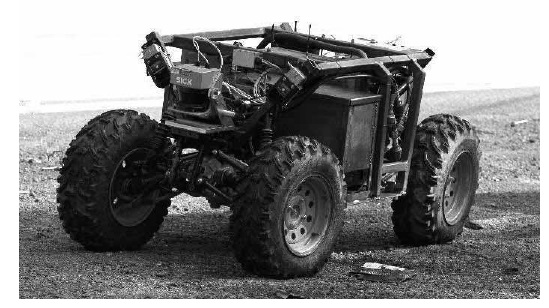
\includegraphics[width=0.7\linewidth]{114orig}}
	\caption{ ( Рис. 11.4 Робор «Groundhog» («Сурок») - 640 килограммовый самоходный робот, оборудованный бортовым компьютером, лазерными датчиками расстояния, датчиками газа и воды, а также системой видеофиксации. Робот был построен для картографирования заброшенных шахт))}
	\label{fig:114orig}
\end{figure}

ОТРИЦАТЕЛЬНАЯ ИНФОРМАЦИЯ \\

Наконец, алгоритм GraphSLAM не принимает в расчёт отрицательную информацию.
На практике отсутствие признака может быть столь же информативным, как и его наблюдение.  Однако, такая простая формулировка не включает необходимых геометрических вычислений.

В практических задачах возможность использовать отрицательную информацию зависит от модели датчика и модель признаков среды. Например, может появиться необходимость вычислить вероятность сцепления признаков, что будет затруднительно для определённых типов датчиков, например, датчики расстояния и направления. Современные реализации, конечно же, учитывают отрицательную информацию, но часто путём замещения чистых вероятностных вычислений приближениями. Один такой пример будет приведён в следующем разделе.\\

\textbf{11.7	Практическая реализация}\\

Обсудим практические реализации GraphSLAM. Мобильный робот, используемый для экспериментов и показанный на Рис. 11.4, предназначен для составления карт заброшенных шахт.

Типовая карта, полученная роботом, показана на Рис. 11.5. Это карта сетки занятости, эффективно использующая попарное сравнение сканирований для восстановления положений робота. Попарное сравнение сканирований можно воспринимать в виде GraphSLAM, но соответствие устанавливается только между двумя последовательными проходами сканирования. Результат использования очевидно показывает недостатки на карте, показанные на Рис. 11.5.

\begin{figure}[H]
	\center{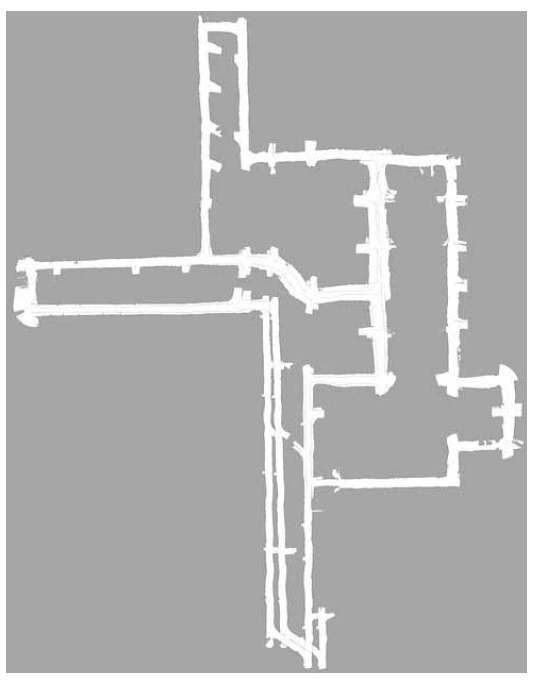
\includegraphics[width=1\linewidth]{115orig}}
	\caption{ ( Рис. 11.5 Карта шахты, полученная попарным сравнением проходов сканирования. Поперечный размер составляет, приблизительно, 250 метров. Карта не целостная, некоторые проходы показаны несколько раз. Изображение принадлежит Дирку Хенелу, университет Фрайбурга (Dirk Hähnel, University of Freiburg).) }
	\label{fig:115orig}
\end{figure}

\begin{figure}[H]
	\center{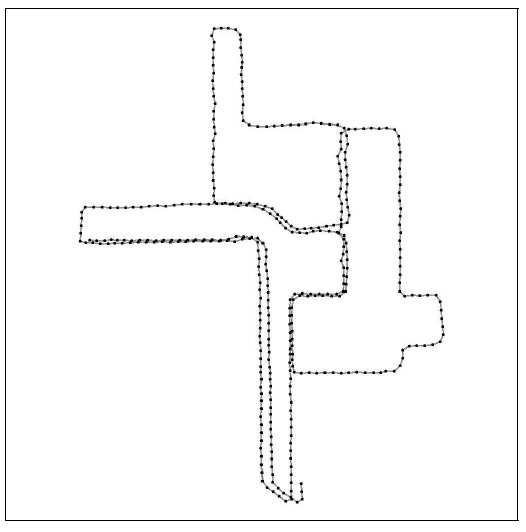
\includegraphics[width=1\linewidth]{116orig}}
	\caption{ ( Рис. 11.6 Основа карты шахты для визуализации локальных карт.) }
	\label{fig:116orig}
\end{figure}

Для использования алгоритма GraphSLAM в нашем программном обеспечении выполняется разбиение карты на мелкие локальные карты, по одной на каждые пять метров движения робота. На протяжении этих пяти метров карты имеют удовлетворительную точность, поскольку общий дрейф показаний мал, и сравнение проходов сканирования происходит, по большей части, гладко. Координаты каждой вспомогательной карты становятся узлом в GraphSLAM. Соседние вспомогательные карты соединяются с помощью относительных ограничений движения между ними. Результирующая структура показана на Рис. 11.6.

\begin{figure}[H]
	\center{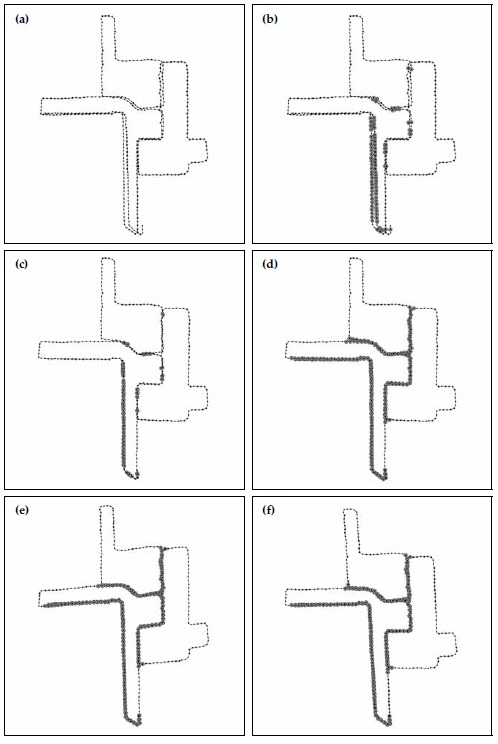
\includegraphics[width=1\linewidth]{117orig}}
	\caption{ ( Рис. 11.7    Поиск ассоциации данных. Пояснения в тексте.) }
	\label{fig:117orig}
\end{figure}

\begin{figure}[H]
	\center{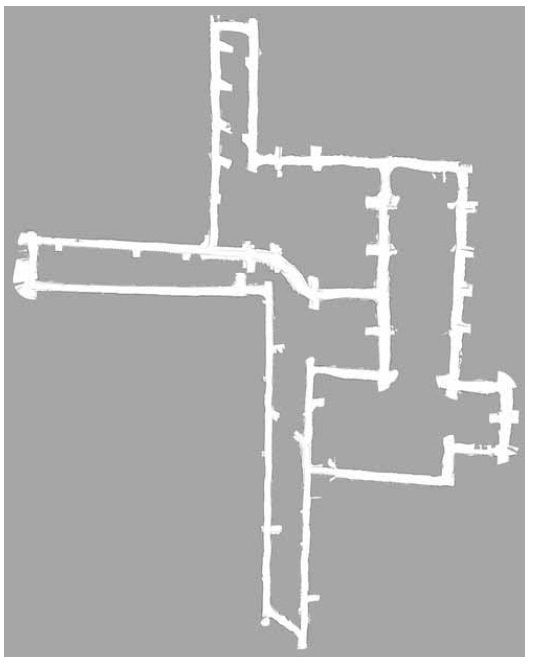
\includegraphics[width=1\linewidth]{118orig}}
	\caption{ ( Рис. 11.8 Итоговая карта после оптимизации ассоциации данных. Изображение принадлежит Дирку Хенелу, университет Фрайбурга (Dirk Hähnel, University of Freiburg).) }
	\label{fig:118orig}
\end{figure}

\begin{figure}[H]
	\center{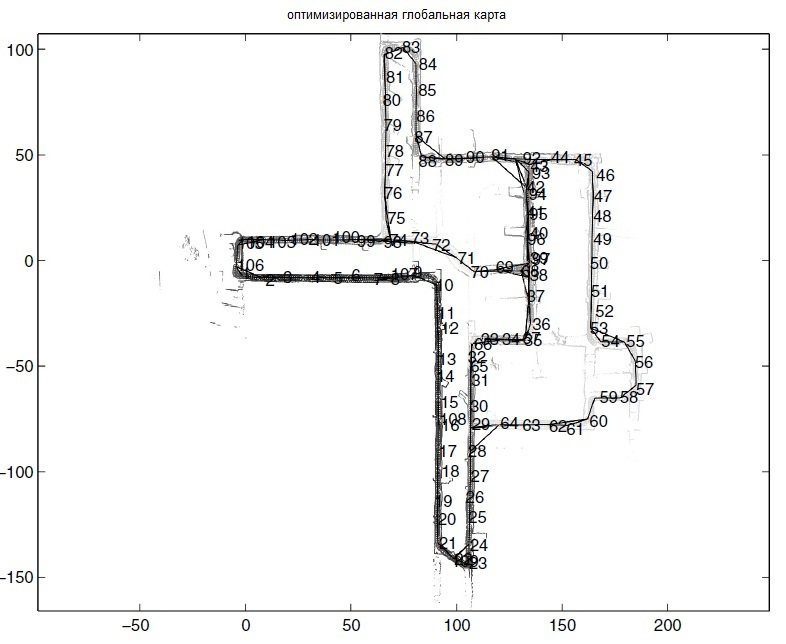
\includegraphics[width=1\linewidth]{119orig}}
	\caption{ ( Рис. 11.9 Карта шахты, сгенерированная алгоритмом Atlas SLAM, созданным Боссе (Bosse et al., 2004). Изображение принадлежит Майклу Боссе, Полу Ньюману, Джону Леонарду и Сету Теллеру, МИТ (Michael Bosse, Paul Newman, John Leonard, Seth Teller, MIT).) }
	\label{fig:119orig}
\end{figure}

Теперь применим рекурсивный поиск ассоциации данных. Проверка соответствия сейчас будет выполняться путём корреляционного анализа двух наложенных друг на друга карт и гауссовых ограничений совпадения, восстановленных аппроксимацией функции совпадения с помощью гауссовых функций. На Рис. 11.7 показан процесс ассоциации данных. Каждый круг соответствует новому ограничению, которое вызывается при конструировании информационного вида с помощью GraphSLAM. На этом рисунке хорошо видна последовательность поиска: некоторые соответствия обнаруживаются только после установления других, а некоторые – удаляются в процессе поиска. Конечная модель стабильна,когда при выполнении поиске новых ассоциаций данных не вносится дальнейших изменений. Двухмерная карта в виде сетки представлена на Рис. 11.8. Хотя эта карта далека от идеальной, в основном из-за грубой реализации ограничений наложения локальных карт, она намного лучше варианта, созданного инкрементным наложением карт.

Читатель может заметить,что другие информационно-теоретические методы SLAM дают сходные результаты. На Рис. 11.9 показана карта на основе того же набора данных, созданного Боссе (Bosse et al., 2004) с помощью алгоритма под названием Atlas. Этот алгоритм разбивает карты на субкарты, отношение между которыми сохраняется в виде относительных информационно-теоретических связей. Более детальная информация приводится в библиографических примечаниях.\\

\textbf{11.8	Альтернативные методы оптимизации}\\

Как читатель может припомнить, центральная целевая функция $J_{GraphSLAM}$ в алгоритме GraphSLAM - это нелинейная квадратичная функция в Выражении (11.3). GraphSLAM минимизирует эту функцию путём последовательных линеаризаций, вычёркивания переменных и оптимизации. Метод предположений в \textbf{GraphSLAM\_solve} в Таблице 11.4, в общем, не слишком эффективен. Если необходимо найти только карту и траекторию пути, без ковариаций, вычисления инверсии в строке 2 в Таблице 11.4 можно избежать. Получившаяся реализация будет намного более вычислительно эффективной.

Ключ к эффективной формулировке  - в функции $J_{GraphSLAM}$. Эта функция в общем, представляет собой метод наименьших квадратов, а значит, может быть минимизирована с помощью различных алгоритмов, описанных в литературе. Примеры включают \textit{методы градиентного спуска, Левенберга-Марквардта, и сопряжённых градиентов}.\\

СОПРЯЖЕННЫЕ ГРАДИЕНТЫ\\

На Рис. 11.10a показаны результаты, полученные с использованием сопряжённого градиента для минимизации $J_{GraphSLAM}$. Данные карты открытого пространства размером примерно 600 на 800 метров были собраны в кампусе  Стенфордского университета роботом, показанным на Рис. 11.10b. На Рис. 11.11 показан процесс выравнивания набора данных, основанного только на информации о положениях робота, до построения полной карты и пути робота. В этом наборе данных содержится приблизительно $10^8$ признаков и $10^5$ положений. Запуск EKF на таком большом наборе данных вряд ли будет разумным, как и инверсия матрицы $\varOmega$ в Таблице 11.4. Методу сопряжённых градиентов потребовалось всего несколько секунд для выполнения минимизации в $J_{GraphSLAM}$. Именно поэтому во многих современных реализациях используются различные способы оптимизации вместо относительно сложных алгоритмов, обсуждаемых в книге. Заинтересованный читатель может обратиться к библиографическим примечаниям с указанием источников, описывающих альтернативные методы оптимизации.

\begin{figure}[H]
	\center{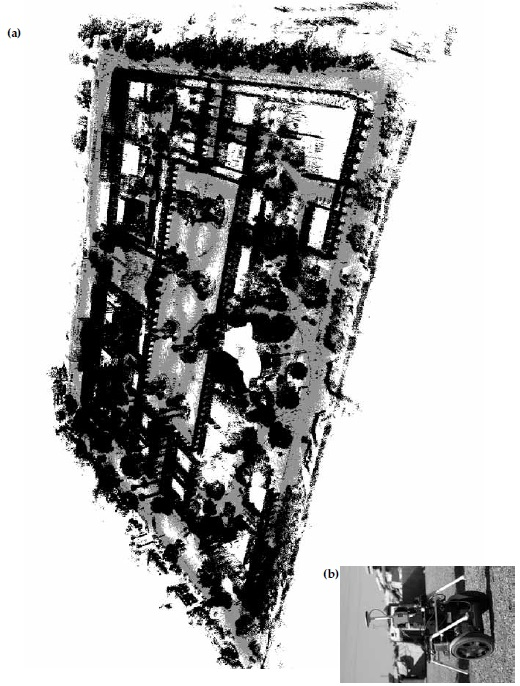
\includegraphics[width=1\linewidth]{1110orig}}
	\caption{ ( Рис. 11.10   Трёхмерная карта кампуса Стэнфорда(a). Робот, используемый для получения этих данных на шасси сегвея RMP, разработка была финансово поддержана программой DARPA MARS(b). Изображение принадлежит Майклу Монтемерло из университета Стэнфорда (Michael Montemerlo, Stanford University). (Страницу следует повернуть вправо.)) }
	\label{fig:1110orig}
\end{figure}

\begin{figure}[H]
	\center{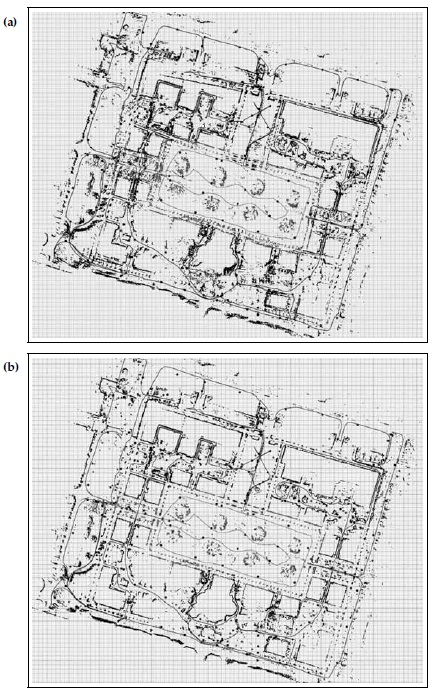
\includegraphics[width=0.9\linewidth]{1111orig}}
	\caption{ ( Рис. 11.11 Двухмерный срез карты кампуса Стэнфорда  до (a) и после выравнивания с помощью метода сопряжённых градиентов (b). Такая оптимизация методом сопряжённых градиентов требует всего нескольких секунд, применительно к формулировке GraphSLAM методом наименьших квадратов. Изображение принадлежат Майклу Монтемерло, университет Стэнфорда (Michael Montemerlo, Stanford University) ) }
	\label{fig:1111orig}
\end{figure}

\textbf{11.9	Выводы}\\

В этой главе описывается алгоритм GraphSLAM для полной задачи SLAM.\\

•	Алгоритм GraphSLAM предназначен для решения полной задачи SLAM. Он вычисляет апостериорные вероятности по всему пути робота и по всей карте. Поэтому, GraphSLAM является пакетным алгоритмом, а не онлайновым, как EKF SLAM.\\

•	GraphSLAM строит граф мягких ограничений на основе набора данных. В частности, измерения проектируются в виде рёбер, представляющих собой нелинейные ограничения между положениями и обнаруженными признаками, а команды на движение представлены в виде мягких ограничений между соседними положениями. Граф изначально разрежен. Количество рёбер является линейной функцией количества узлов, и каждый узел соединён с конечным количеством других узлов независимо от размера графа.

GraphSLAM просто сохраняет всю информацию в графе с помощью связей, определённых между положениями и признаками, а также между парами последовательных положений. Однако, это информационное выражение не даст оценок карты или пути робота.\\

•	Сумма всех ограничений задана функцией $J_{GraphSLAM}$. Оценки максимального правдоподобия для пути робота и карты могут быть получены минимизацией функции $J_{GraphSLAM}$.\\

•	GraphSLAM выполняет проекцию графа в виде изоморфной информационной матрицы и информационного вектора, определённых по всем положениям пути и всей карте. Ключевой идеей алгоритма GraphSLAM является разрежённость структуры представления информации. Измерения дают информацию о признаке относительно положения робота в момент измерения. В информационном пространстве они образуют ограничение между парами переменных. Похожим образом, движение несёт информацию о взаимосвязи двух последовательных положений. В информационном пространстве каждая команда на движение образует ограничение между последовательными положениями. Эта разрежённость наследуется из разреженного графа.\\

•	Чистый алгоритм GraphSLAM восстанавливает карты с помощью итеративной процедуры из трёх шагов: построение линейного информационного вида с помощью разложения в ряд Тейлора, уменьшения размера представления для извлечения карты, и решения результирующей проблемы оптимизации по положениям робота. Эти три шага эффективно разрешают информацию и создают целостное вероятностное апостериорное распределение по пути робота и карте. Поскольку GraphSLAM выполняется пакетно, шаг линеаризации можно повторить для улучшения результата.\\

•	В альтернативных реализациях  вывод выполняется с помощью оптимизации методом наименьших квадратов функции JGraphSLAM. Однако, такие методы позволяют найти только моду апостериорной вероятности, но не её ковариацию.\\

•	Ассоциация данных в GraphSLAM выполняется вычислением вероятности того, что два признака имеют идентичные координаты в среде. Поскольку GraphSLAM – пакетный алгоритм, его можно выполнять для любой пары признаков, в любое время. Это приводит к итеративному жадному алгоритму поиска по всем переменным ассоциации данных, рекурсивно определяющим пары признаков на карте с наибольшим значением соответствия.\\

•	В практических реализациях GraphSLAM часто используются дополнительные приёмы уменьшения количества вычислений и предотвращения ошибочных ассоциаций данных. В частности, на практике стремятся уменьшить сложность данных, извлекая локальные карты и используя каждую карту в качестве базового элемента картографирования. В таких методах сравниваются несколько признаков за проход, и есть возможность учитывать отрицательную информацию при выполнении поиска ассоциации данных.\\

•	Были кратко представлены результаты GraphSLAM на основе декомпозиции, но использующего карты сеток занятости для представления наборов данных расстояния. Несмотря на эти приближения, было обнаружено, что методы ассоциации данных и вывода карт демонстрируют лучшие результаты в масштабных задачах картографирования.\\

•	Также были представлены результаты для реализации метода сопряжённого градиента в задаче наименьших квадратов. Было замечено, что общая целевая функция GraphSLAM может быть оптимизирована методом наименьших квадратов. Некоторые методы, например, сопряжённый градиент, существенно быстрее по сравнению с базовым методом оптимизации в GraphSLAM.\\

Как было замечено во вводной части, EKF SLAM и GraphSLAM расположены на противоположных сторонах диапазона SLAM алгоритмов. Алгоритмы, которые попадают между этими крайними значениями, будут обсуждаться в следующих двух главах. Ссылки на такие методы находятся в библиографических примечаниях нескольких следующих глав.\\

\textbf{11.10	Библиографические примечания} \\

Методы графического представления хорошо известны в машинном зрении и фотограмметрии и относятся к структуре из движения и блочного выравнивания (Hartley and Zisserman 2000; B et al. 2000; Mikhail et al. 2001). Первые упоминания об относительных ограничениях в виде графа в литературе по SLAM восходят к работам Чизмана и Смита (Cheeseman and Smith, 1986) и Дюран-Уайта (Durrant-Whyte, 1988), но в этих подходах не было оптимизации. Представленный в этой главе алгоритм произвольно основан на основополагающей работе Лю и Милиоса (Lu and Milios, 1997). Исторически, они первые выразили априорную вероятность SLAM в виде набора связей между положениями робота, сформулировав алгоритм глобальной оптимизации для генерации карты на основе набора ограничений. Их оригинальный алгоритм для глобального выравнивания целостных сканирований расстояния использовал переменные положения робота как систему отсчёта, что отличалось от стандартной точки зрения EKF, в которой положения интегрировались. Используя анализ данных одометрии и сканирования расстояния лазером, их метод создавал относительные ограничения между положениями, которые можно рассматривать аналогично рёбрам в GraphSLAM. Однако, они не сформулировали метод в информационном представленим. Алгоритм Лю и Милиоса (1997) был впервые успешно реализован Гутманом и Небелем (Gutmann and Nebel, 1997), которые отметили вычислительную неустойчивость, возможно, из-за излишнего использования инверсии матриц. Голфарелли (Golfarelli et al., 1998) первым установил связь задач SLAM и кинематических моделей на основе масс и пружин, а Дакитт (Duckett et al., 2000, 2002) представил первый эффективный метод решения таких задач. Отношение между ковариацией и информационной матрицей обсуждалось в работе Фризи и Хирзингера (Frese and Hirzinger, 2001). Аранеда (Araneda, 2003) разработал более детальную и точную графическую модель.

Алгоритм Лю и Милиоса положил начало разработке оффлайновых алгоритмов SLAM, которые, до настоящего времени, развиваются почти параллельно работам по EKF. Гутманн и Конолиг (Gutmann and Konolige) объединили эту реализацию с шагом марковской локализации для установки соответствия при замыкании петель в циклической среде. Босси (Bosse et al., 2003, 2004) разработал алгоритм Atlas, иерархическую картографическую систему на основе парадигмы разделённого стохастического картографирования, сохраняющего относительную взаимосвязь между вспомогательными картами. В нем используется метод оптимизации, похожий на предложенный Дакиттом (Duckett et al.,2000) и на GraphSLAM с выравниванием нескольких карт.  Фолькессон и Кристенсен (Folkesson and Christensen, 2004a,b) раскрыли перспективу оптимизации SLAM, применив версию градиентного спуска к логарифму правдоподобия апостериорного распределения. Их алгоритм Graphical SLAM уменьшал число переменных для пути, так же как GraphSLAM, при замыкании петли. Это уменьшение (математически являющееся приближением, поскольку выполнялось отбрасывание карты) существенно ускорило выполнение градиентного спуска. Конолиг (Konolige, 2004) и Монтемерло и Трун  (Montemerlo and Thrun, 2004) представили сопряжённый градиент в области SLAM, который показал как большую эффективность по сравнению с градиентным спуском. В обеих работах  количество переменных при закрытии больших циклов уменьшалось, что позволяли выравнивать карты с $10^8$ признаков всего за несколько секунд. Метод Левенберга-Маркардта, упомянутый в тексте, принадлежит Левенбергу (Levenberg, 1944) и Маркардту (Marquardt, 1963), которые вывели его в контексте оптимизации вычисления методом наименьших квадратов. Фризи (Frese et al., 2005) проанализировал эффективность SLAM в информационном виде, и разработал высокоэффективные методы оптимизации, используя оптимизацию нескольких сеток. Он отметил увеличение скорости на несколько порядков, и эти методы оптимизации в настоящее время являются наиболее совершенными. Делаэрт (Dellaert, 2005) разработал эффективные методы факторизации для графа ограничений GraphSLAM, направленные на преобразование графа ограничений в более компактные версии, сохраняя разрежённость.

Следует отметить, что идея сохранения относительных связей между локальными элементами лежит в основе многих методов на основе вспомогательных карт, описанных в предыдущем разделе, хотя и редко в явном виде. Рядом автором, среди которых Гювант и Небот (Guivant and Nebot, 2001), Вильямс (Williams, 2001), Тардос (Tardós et al., 2002), Бейли (Bailey, 2002) были описаны структуры данных для относительных смещений между вспомогательными картами, которые легко укладываются в информационные теоретические концепции. Хотя многие из этих алгоритмов являются фильтрами, они разделяют многие общие идеи информационного представления, обсуждаемого в этой главе.

Насколько нам известно, алгоритм GraphSLAM, представленный здесь, никогда не публиковался в указанном виде (в раннем черновике этот алгоритм называется "расширенным информационным видом"). Однако, GraphSLAM тесно связан с публикациями, указанными ранее, и основан на фундаментальном алгоритме Лю и Милиоса (1997). Название GraphSLAM напоминает название Graphical SLAM, использованное Фолкенссоном и Кристенсеном (2004a). Оно было выбрано для этой главы, поскольку графы ограничений являются основой всего направления исследований SLAM. Множество авторов разработали фильтры в информационном виде, которые решают онлайн задачу SLAM вместо полной задачи SLAM. Эти алгоритмы будут обсуждаться в следующей главе, полностью посвящённой проблеме фильтрации.

Формулировка GraphSLAM проблемы SLAM основана на десятилетнем обсуждении выражения пространственных карт, которые уже упоминались в библиографических примечаниях к Главе 9. Информационные представления сводят вместе две разные парадигмы представления карт: топологическую и метрическую. Дебаты о представлении пространства для людей и роботов остались позади  (Chown et al. 1995). Топологические подходы уже обсуждались в библиографических примечаниях к Главе 9. Ключевым свойством топологического представления является факт отображения только относительной информации между элементами карты. Поэтому в них отсутствует проблема нахождения целостного метрического обоснования этой относительной информации. В наиболее современных топологических методах связи между элементами дополняются метрической информацией, такой как расстояние между двумя местоположениями.

Так же как в топологических представлениях, информационно-теоретические методы накапливают относительную информацию между соседними объектами (ориентирами и роботами). Но относительная линейная информация карты «переводится» в метрическое обоснование. В случае использования линейной гауссовой функции, шаг вывода не теряет информацию и, поэтому, обратим. Вычисление полной апостериорной вероятности, включая ковариацию, требует обращения матриц. Вторая операция обращения матриц ведёт к начальной форме относительных ограничений. Поэтому, топологический и метрический вид дополняют друг друга, так же как информационно-теоретическое и вероятностное представления (или EKF и GraphSLAM). Так может, стоит объединить математический и подход, чтобы соединить вместе топологические и метрические карты? Читателю следует знать, что такая точка зрения ещё не распространилась среди большинства исследователей.\\

\textbf{11.11	Упражнения}\\

1.	В предыдущей главе в упражнениях уже использовалось \textit{SLAM только по направлению}, как разновидность SLAM, в которой датчики способны измерять только направление на ориентир, но не расстояние до него. Мы предполагаем, что GraphSLAM лучше подходит для этой задачи, чем EKF. Почему?\\

2.	В этом вопросе, требуется доказать сходимость результатов для особого класса проблем SLAM: \textit{SLAM в виде линейных гауссианов}.\\
SLAM В ВИДЕ ЛИНЕЙНЫХ ГАУССИАНОВ\\
В SLAM в виде линейных гауссианов, уравнение движения имеет простой аддитивный вид\\

$$x_t\sim\mathcal{N}(x_{t-1}+u_t,R)$$

а уравнение измерений - вид\\

$$z_t=\mathcal{N}(m_j-x_t Q)$$

где $R$ и $Q$ - диагональные матрицы ковариации, а $m_j$ признак, наблюдаемый в момент времени $t$. Можно допустить, что количество ориентиров конечно, все ориентиры наблюдаются бесконечно часто и без определённого порядка, а соответствия - известны.\\

(a)	Доказать, что для GraphSLAM расстояние между любыми двумя ориентирами сводится к верному с вероятностью 1.\\

(b)	Как это доказательство относится к EKF SLAM?\\

(c)	Подходит ли GraphSLAM для общей задачи SLAM с известным соответствием? Если да, объяснить, почему, если нет – тоже объяснить (без доказательства).\\

3.	Алгоритм \textbf{GraphSLAM\_reduce} уменьшает набор ограничений, интегрируя переменные карты, и сохраняя систему ограничений только по положениям робота. Возможно ли вместо этого интегрировать положения робота, так, чтобы результирующая сеть ограничений была определена исключительно по переменным карты? Если да, будет ли результирующая задача вывода разреженной? Как циклы на пути робота повлияют на новый набор ограничений?\\

4.	Алгоритм GraphSLAM в этой главе игнорирует сигнатуры ориентиров. Расширить базовый алгоритм GraphSLAM для использования сигнатур в измерениях и на карте.\\










 
\end{document}